\documentclass[12pt,a4paper]{scrartcl}
\usepackage{geometry}
\usepackage[ngerman]{babel}
\usepackage[T1]{fontenc}
\usepackage{slashbox}
\usepackage{verbatim} %mehrzeilige Kommentare
\usepackage{url}
\usepackage[bottom,hang]{footmisc}
\usepackage[onehalfspacing]{setspace}
%\usepackage{hyperref}
\usepackage[breaklinks=true]{hyperref}
\usepackage{cite}
%\usepackage{bibgerm}
%\usepackage{natbib}
\usepackage{blindtext}
\usepackage[utf8]{inputenc} %ä,ö,ü
\usepackage{amsmath} %Mathematischer Formelsatz
\usepackage{amsfonts} %Mathesymbole
\usepackage{amssymb} %Mathesymbole
\usepackage{setspace}
\usepackage{geometry}
\usepackage{tabularx, calc} %Tabellen
%\usepackage{acronym} %Abkürzungsverzeichnis
\usepackage{color} % Farbe
%\usepackage{titlesec}
\usepackage{graphicx} %Graphiken einfügen
\usepackage[automark, headsepline, footsepline, ilines]{scrpage2} %Kopf- und Fußzeilen
\usepackage{multirow} %Tabelle: mehrere Spalten vereinigen
\usepackage{calc} %Rechnungen
%\usepackage{booktabs} %Verbesserung der Tabellenqualität
\usepackage{tabularx, calc} %Tabellen
\usepackage{longtable} %Tabelle über mehrere Seiten
\usepackage{textcomp} %Sonderzeichen
\usepackage{lmodern} %modernisierte Schriftart
\usepackage{booktabs}
\usepackage{multirow}
\usepackage{ragged2e}
\usepackage{float} % erwzingt Bildposition wo man will z.B H = here

\deffootnote{1.7em}{2.7em}{{\scriptsize\thefootnotemark~~}} 
\addtokomafont{footnote}{\RaggedRight}
%\usepackage{subfigure}
%\usepackage[square]{natbib} %Literaturverzeichnis für naturwissenschaftliche Arbeiten
%\usepackage{wolke} %Abbildungsunterschrift und Tabellenüberschrift mit Kapitelzahl z.B. Abb.: 1.1
%\usepackage{picinpar} %Bild im Text
%\usepackage{picins} %Bild im Text
%\usepackage{caption} %Abbildungs- und Tabellenbeschriftung
%\usepackage{array} %Matheumgebung ähnlich tabular
%\usepackage{dcolumn} %tabelle:kommata untereinander
\titlehead{
\includegraphics[width=5cm]{euletext.png} \hfill 
\includegraphics[width=6cm]{semvox2.png} }
%\titlehead{
\includegraphics[width=7cm]{euletext.png} \hfill}
 %Titelkopf
\title{$\,$\\  Disambiguierungsstrategien in Dialogsystemen}
\rohead{\leftmark}\cohead{} %Kopfzeile: Kapitelüberschrift rechts, nicht mitte
\setlength{\parindent}{0pt} %ohne Einrückung
%\captionsetup{font={footnotesize,bf}} %Abbildungs-und Tabellenbeschriftung klein und fett
\date{}
\setlength{\headsep}{1,25cm} %Abstand zwischen Kopfzeile und Text
%\titlespacing{\section}{0pt}{*1}{1.3cm} 
\author{}
\linespread{1,5} %Zeilenabstand
\clubpenalty10000 % Hurenkinder und Schusterjungen verhindern
\widowpenalty10000 % Hurenkinder und Schusterjungen verhindern
\displaywidowpenalty=10000 % Hurenkinder und Schusterjungen verhindern
\newenvironment{myitemize}{\begin{itemize}\itemsep -2pt}{\end{itemize}}
\pagestyle{scrheadings}
%\setlength{\heavyrulewidth}{1pt} %Tabularx: Dicke der Linien
%\setcounter{tocdepth}{5} %Tiefe des Inhaltsverzeichnisse: 4: section, subsection, subsubsection + paragraph 								im Inhaltsvereichnis
%\setcounter{secnumdepth}{5} %bis zu welcher Schachtelungstiefe erfolgt die Nummerierung des 												Inhaltsverzeichnisses 4: bis paragraph
%\setlength{\tabcolsep}{8pt}
%  \renewcommand\appendix{\par 
%    \setcounter{section}{0}
%    \setcounter{subsection}{0} 
%    \renewcommand\thesection{\Alph{section}}		%alphabetische Nummerierung der Überschriften im Anhang
%    \renewcommand\thefigure{\Alph{section}\arabic{figure}}} %Nummerierung der Abbildungen im Anhang
%	\renewcommand{\arraystretch}{1,5}    
    
\begin{document}
\pdfoutput=1
\pagenumbering{Roman}


\maketitle
\sffamily
\begin{center}
\huge
\textbf{Bachelorarbeit}\\
\vfill
\LARGE
Fachrichtung Computerlinguistik\\
\vfill
\normalsize
vorgelegt von\\
\Large
\textbf{Lena Enzweiler}\\
\vfill


\normalsize
Bachem,
\today

\end{center}

\thispagestyle{empty}
\rmfamily
\cleardoublepage


%\begin{comment}
\section*{Eidesstattliche Erklärung}

%\cfoot{}
\markboth{Eidesstattliche Erklärung}{Eidesstattliche Erklärung}
Ich versichere, die Bachelorarbeit selbstständig und lediglich unter Benutzung der angegebenen Quellen und Hilfsmittel verfasst zu haben.
\newline
\newline
Ich erkläre weiterhin, dass die vorliegende Arbeit noch nicht im Rahmen eines anderen Prüfungsverfahrens eingereicht wurde.
\newline
\newline

Bachem, \today
%\thispagestyle{empty}
\newpage
%\end{comment}

%\begin{comment}
\section*{Danksagung}
\markboth{Danksagung}{Danksagung}
An dieser Stelle möchte ich mich bei allen bedanken, die mich während der Anfertigung dieser Bachelorarbeit fachlich und persönlich unterstürzt haben.\\



Ich möchte mich zunächst bei Herrn Prof. Dietrich Klakow für die Überlassung des interessanten Themas bedanken.\\
\\
Mein Dank gilt ganz besonders der Semvox GmbH und ihren Mitarbeitern, ohne die diese Arbeit nicht möglich gewesen wäre. Insbesondere danke ich Pia Kuznik, Dr.-Ing. Markus Löckelt und Jan Schehl für die Bereitstellung dieses interessanten Themas, die ständig freundliche Hilfsbereitschaft und für all die nützlichen Tipps zur Anfertigung dieser Arbeit. 
Pia Kuznik möchte ich außerdem ganz herzlich für die nette und engagierte Betreuung meiner Bachelorarbeit bedanken.\\
\\
Ein ganz besonderer Dank gilt allen Personen, die sich mir als Versuchsperson und Korrekturleser zur Verfügung
gestellt haben.\\
\\
Ganz besonders möchte ich mich bei Christine Braun bedanken, die mir durch kritisches Hinterfragen und konstruktive Kritik immer wieder wertvolle Hinweise gab. Weiter möchte ich mich für die nützlichen Tipps zur Gestaltung meiner Arbeit bedanken.\\
\\
Bei Tobias Aggintus möchte ich mich herzlich für die stetige Aufmunterung, alltägliche Unterstützung und Hilfe während der gesamten Studienzeit bedanken. \\
\\
Mein ganz besonderer Dank gilt abschließend meiner Familie, insbesondere meiner Mutter, meiner Schwester, Vitter und Katja für die moralische und finanzielle Unterstützung während meines gesamten Studiums. \\
%\cfoot{}
\markboth{Danksagung}{Danksagung}
%\thispagestyle{empty}
\cleardoublepage
%\end{comment}

$\,$\\
\vfill
\markboth{ }{ }
Meine Bachelorarbeit entstand im Zeitraum vom September 2014 bis Oktober 2014 bei SemVox GmbH unter der Leitung von Prof. Dietrich Klakow und der Betreuung von Pia Kuznik.


\cleardoublepage




\cleardoublepage
\tableofcontents
\cleardoublepage

\markboth{Abkürzungsverzeichnis}{Abkürzungsverzeichnis}
\addcontentsline{toc}{section}{Abkürzungsverzeichnis}
\section*{Abkürzungsverzeichnis} 
\cleardoublepage
\begin{comment}
\addcontentsline{toc}{section}{Abbildungsverzeichnis}
\listoffigures
\cleardoublepage

\addcontentsline{toc}{section}{Tabellenverzeichnis}
\listoftables
\cleardoublepage
 


\cleardoublepage



\end{comment}


\pagenumbering{arabic}

\renewcommand{\abstractname}{Abstract}
\markboth{Abstract}{abstract}
\subsection*{\centering {Abstract}}  
\begin{abstract}
Die vorliegende Arbeit beschäftigt sich mit der Frage, welche Disambiguierungsstrategien in Sprachdialogsystemen für Benutzer bei hoher kognitiver Belastung am geeignetsten sind. Man fokussiert sich dabei auf Sprachdialogsysteme, welche speziell für die Bedienung während der Autofahrt konzipiert werden. Um der Frage der besten Disambiguierungsstrategie nachzugehen, werden in einem Wizard-of-Oz-Experiment Fahrszenarien simuliert, bei denen die Versuchspersonen mit einem Dialogsystem sprachlich interagieren. Dabei werden ambige Eingaben des Benutzers simuliert worauf das System mit Disambiguierungsstrategien in Form von Nachfragen reagiert. Diese verlangen eine entsprechende Benutzerreaktion. Anhand der Versuchsergebnisse wird analysiert, welche Strategien für den Benutzer am einfachsten zu benutzen und effektivsten waren. Insgesamt werden drei Disambiguierungsstrategien verfolgt. Aggregierte Auswahl ohne Pause, aggregierte Auswahl mit Pause, sowie die sequentielle Auswahl. Bei der aggregierten Auswahl ohne Pause werden alle möglichen Interpretationen einer ambigen Spracheingabe nacheinander in einer Sprachausgabe ausgegeben. Die aggregierte Auswahl mit Pause gibt alle möglichen Interpretationen durchnummeriert und durch Pausen getrennt in einer Sprachausgabe aus. In der sequentiellen Ausgabe wird jede Interpretation in einer separaten Sprachausgabe formuliert.   
\end{abstract}
\newpage
\section{Einleitung}

Dialogsysteme im automobilen Bereich müssen so gestaltet werden, dass sie den Fahrer so wenig wie möglich vom Fahren ablenken und ihm so gut wie möglich assistieren. Die Herausforderung für einen Entwickler von Sprachdialogsystemen (Dialogdesigner) besteht daher darin, Sprachäußerungen raffiniert zu gestalten. Dabei müssen dem Benutzer alle relevanten Informationen in verständlicher Weise geliefert werden. Darauf sollte möglichst einfach geantwortet und Anfragen und Wünsche effizient übermitteln werden können. Die Funktionsweise eines Dialogsystems hängt von mehreren Komponenten ab, welche anhand der in Abbildung \ref{odps3} dargestellten Funktionsweise der Semvox GmbH eigenen ODP S3 Plattform \footnote{\label{foot:odps3}\url{http://www.semvox.de/de/technologie/odp-s3.html}} kurz erläutert werden. Die ODP S3 Plattform ermöglichst die Umsetzung komplexer Sprachdialoge, indem Spracheingaben eines Benutzers als semantische Objekte behandelt werden. Dabei wird eine Spracheingabe mit einer Backus-Naur-Form (BNF) Grammatik interpretiert, welche alle möglichen Spracheingaben des Benutzers listet und semantischen Objekten zuweist. BNF ist eine Metasprache, mit welcher bestimmt werden kann, ob eine Spracheingabe valide ist (\cite{BNFref}). Semantische Objekte werden von einem Backend-Server verarbeitet, woraufhin eine passende Sprachausgabe generiert wird. 
\begin{figure}[htbp]
\begin{center}
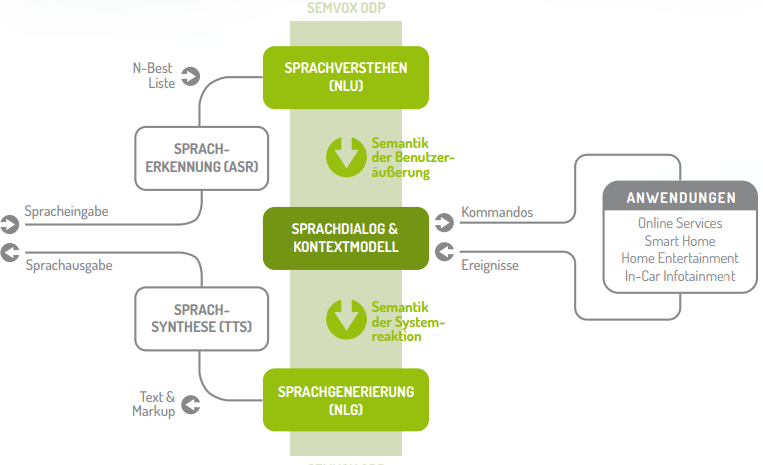
\includegraphics[width=12cm]{odps3.png}
\caption{Funktionsweise der ODP S3 Plattform}
\label{odps3}
\end{center}
\end{figure}
\newline
\newline
In dieser Arbeit konzentriert man sich allein auf die Sprachgenerierung. Ein komplexer Dialog zwischen System und Benutzer führt häufig dazu, dass der Benutzer eine Eingabe macht, die das System nicht eindeutig zuordnen kann und mehrere Optionen für die Interpretation der vom Benutzer geäußerten Eingabe bestehen. Es muss an dieser Stelle vom System eine Rückfrage beim Benutzer erfolgen, sodass dieser seine vorherige Eingabe eindeutig übermitteln kann. Wenn der Benutzer zum Beispiel den Wunsch äußert einen Kontakt aus dem im System gespeicherten Adressbuch anzurufen, es allerdings zwei Kontakte mit diesem Namen gibt, muss das System eine Rückfrage stellen, um zu ermitteln, welcher dieser beiden Kontakte gemeint ist. Der Dialogdesigner spricht in diesem Fall von Disambiguierung.  Es wird in der vorliegenden Arbeit der Frage nachgegangen wie man konkret die Sprachausgabe einer solchen Disambiguierung innerhalb eines Dialogsystems, das speziell im Rahmen einer automobilen Anwendung konzipiert wird, gestaltet. Dabei werden drei verschiedene Strategien in einem Experiment auf Effizienz und Beliebtheit unter den Versuchspersonen getestet. Diese Strategien werden im Kapitel \ref{disambiguierungsstrategien} (Disambiguierungsstrategien) näher erläutert. Da für diesen Versuch kein Dialogsystem implementiert und lediglich ein Control Panel entwickelt wurde, das die Sprachausgaben eines Systems simuliert, handelt es sich bei dem Versuch um ein Wizard-of-Oz Experiment. Dabei wird den Versuchspersonon mitgeteilt, dass sie mit einem echten Dialogsystem interagieren und wissen nicht, dass die Sprachausgaben vom Versuchsleiter gesteuert werden (siehe \ref{WOZ} Wizard-of-Oz). Der Versuch in Kapitel \ref{versuch1}  (Versuch1) zeigt klar, dass bei einer Disambiguierung über wenige mögliche Slotfüller die Strategie \texttt{Aggregierte Auswahl ohne Pause} am beliebtesten unter den Versuchsperson ist. Es wurde sich für einen zweiten Versuch entschieden, welcher sich lediglich in der Länge der Disambiguierung unterscheidet. Dieser in Kapitel \ref{Verusch2} (Versuch2) durchgeführte Versuch zeigt, dass bei einer Disambiguierung über mehrere möglichen Slotfüller die Strategie \texttt{Sequentielle Auswahl} die beliebteste Strategie ist. Neben der Beliebtheit unter den Versuchspersonen wurden bei beiden Versuchen weitere Faktoren, wie Dialogzeit, erfolgreiches Abschließen des Dialoges (Task Completion) oder Unterschiede des Dialogverhaltens zwischen hoher und geringer kognitiver Belastung erforscht. Ein zusammenfassendes Ergebnis beider Versuche findet sich in Kapitel \ref{Ergebnisse} (Ergebnisse). Daran schließt sich eine Diskussion über die ermittelten Daten an, mit einem Ausblick für zukünftige Arbeiten. 

\begin{comment}
Bei Autofahrt effektive Sprachsteuerung wichtig \\
dem System darf keine 100prozentige Aufmerksamkeit geschenkt werden\\
Aufbau Dialogsysteme anhand von ODP-s3\\
Disambiguierung oft notwendig (speziell bei Navigierung)\\
für reibungslosen Dialogverlauf --> gute Disambiguierungsstrategie notwendig\\
Fragestellungen:\\
Welche Disambiguierung bei CL + am effektivesten?(bessere Zeit, weniger Fehler, höhere Bewertung)\\
Unterschied kleine versus große Auswahl\\
beeinflusst CL+ das Dialogverhalten? (Reaktionszeit)\\
Allg Unterschiede Cl+ vs Cl- \\
\end{comment}


\begin{comment}
Überblick Dialogsystem\\
DICO (in Dialogue behaviour under high cognitive load)\\
IDIS to meassure CL as to behaviour during driving(in Dialogue behaviour under high cognitive load)
ODP-S3\\
Fließdiagramm\\
Bei Autofahrt effektive Sprachsteuerung wichtig \\
dem System darf keine 100prozentige Aufmerksamkeit geschenkt werden\\
Disambiguierung oft notwendig (speziell bei Navigierung)\\
für reibungslosen Dialogverlauf --> gute Disambiguierungsstrategie notwendig\\
beeinflusst CL das Dialogverhalten?\\
"we believe that our results are still useful as a basis
for future implementation and experimental work."\\
with the goal of designing
interfaces that will help reduce the user’s overall cognitive load.\\
We adopted a “Wizard of Oz” (WOz) approach [2], where the
subject talks to what appears to be an automatic system, but the
system’s responses are in fact generated by a human (the “wizard”)
in another room. This approach allows eliciting high quality
dialog while setting appropriate expectations for the subject
in terms of language complexity, because humans usually
use simpler language when talking to a machine, and therefore
avoids the need for automatically understanding unconstrained
language. This also filters out the conversations irrelevant to
in-car tasks which may occur in human-human interactions. (Mishra et al. )\\ 
\end{comment}


\newpage
\section{Related Work}

Dialogsysteme, Disambiguierungsstrategien in Interaktionen sowie kognitive Belastung von Videospielen in Verbindung mit Dialogsystemen sind Themen, die im Bereich der Computerlinguistik in diversen Arbeiten untersucht werden. Im Folgenden werden einige dieser Arbeiten vorgestellt. \\
\\
Minker et al. untersuchten in einer Studie von 2012 eine weitere Disambiguierungsstrategie für Dialogsysteme. Übermittelt der Benutzer zum Beispiel bei der Navigation eine ambige Stadt als Zielort, fragt das System bei dieser Strategie nach dem ZIP-Code, um die Mehrdeutigkeit aufzulösen. \\
In den Studien von Tsiakoulis et al. von 2012 und Ang et al. von 2006 wurde die kognitive Belastung während Videospielen untersucht. Die kognitive Belastung während einer Systeminteraktion wurde weiter von Tsiakoulis et al. von 2012 und Villing 2009 erforscht. Dabei wurde festgestellt, dass eine kognitive Belastung das Dialogverhalten ändert. Die Ergebnisse zeigen, dass während einer hohen kognitiven Belastung vom Benutzer längere Pausen zwischen zwei Sprachäußerungen eingelegt werden und die Anzahl der Sprachäußerungen geringer sind im Vergleich zur Anzahl während einer niedrigen kognitiven Belastung (\cite{DbCL}).
\cite{eCLDS} kamen zu dem Ergebnis, dass das System während einer hohen kognitiven Belastung öfter durch sprachliche Äußerungen unterbrochen wurde (Barge-in) als bei niedriger Belastung.
In \cite{eCLDS} hat man weiter herausgefunden, dass Versuchspersonen unter kognitiver Belastung Dialogabläufe mit einfachen Spracheingaben wie \texttt{ja} oder \texttt{nein} solchen Dialogabläufen bevorzugen, in denen das System den zu füllenden Slot als Antwort verlangt. Daher wird vermutet, dass die sequentielle Auswahl in dem hier vorgestellten Versuch bei Versuchspersonen mit hoher kognitiver Belastung am effizientesten ist.  In der erwähnten Studie fuhren die Versuchspersonen ebenfalls parallel zur Dialoginteraktion ein Rennspiel. Man hat dabei festgestellt, dass die Task Completion des aufgestellten Tasks bei der alleinigen Interaktion mit dem System höher war als bei der Interaktion parallel zum Rennspiel. Des Weiteren wurde herausgefunden, dass die Versuchspersonen einen Unterschied der kognitiven Belastung zwischen dem alleinigen Fahren, der alleinigen Interaktion und des Fahrens während der Interaktion festgestellt haben. Ähnliche Ergebnisse werden für die vorliegende Studie erwartet. \\
In Ang et al. von 2006 wurde erforscht, dass eine kognitive Belastung, die durch eine parallele Interaktion mit anderen Spielern in einem Computerspiel ausgelöst wird, die Leistung im Spiel verschlechtert.  Die Kommunikation mit anderen Spielern im Computerspiel kann mit der Systeminteraktion aus dieser Studie verglichen werden. Deshalb wird für diese Studie eine schlechtere Rennspielleistung während des Testszenarios im Vergleich zur Rennspielleistung ohne Systeminteraktion erwartet. Dies könnte in zukünftigen Arbeiten überprüft werden.\\
 In \cite{Wozhcd} konnte festgestellt werden, dass Benutzer, die sich mehr auf einen anderen Task als auf die Systeminteraktion konzentrieren, eher unflüssige und abgehackte Sprachausgaben produzieren. In einer zukünftigen Arbeit könnte überprüft werden, ob solche Sprachäußerungen die angewendeten Disambiguierungsstrategien in einem echten System negativ beeinflussen.
Des Weiteren kann diese Erkenntnis dazu genutzt werden, um die Stärke der Ablenkung durch das Rennspiel der einzelnen Versuchspersonen zu bewerten. 

\begin{comment}
\begin{enumerate}
\item [DISAM]\texttt{intelligent dialog strategy for accesssing infotainment applications in mobile environments}
\begin{itemize}
\item System frägt nach Infos zur Disambiguierung. PLZ, Region, nahe Städte, etc
\item Future Work: anderen Disambiguierungsstrategie $\rightarrow$ wo wohnt denn Peter?
\end{itemize}
\item [CL]\texttt{Cognitive Load Issues in MMORPGs}
\begin{itemize}
\item verschiedene Cognitive Loads beschrieben (Interface, Chat, NPC,...)
\item Herangehensweise für Spielaufbau interessant
\item CL in Mario Kart mit CL in MMORPGs zu vergleichen?!
\end{itemize}
\item [CL]\texttt{Automatic Cognitive Load Detection from Speech 
Features}
\begin{itemize}
\item \glqq Analysis of the subjective ratings from the
subjects showed that the designed levels of load were actually
 by the users and consequently could affect their
speech production as hypothesized.\grqq\\
$\rightarrow$ könnte genutzt werden um zu analysieren ob CL vorliegt/wie hoch CL ist
\item \glqq The ability to implicitly measure the perceived level
of cognitive load through changes in multimodal behaviour,
particularly speech, could play a crucial role in human
computer interaction design, applications could adapt the
output flow and presentation to the current load of the user
without intrusive probes.\grqq\\
$\rightarrow$ Future Work: Direkt Strategien auf CL anpassen
\end{itemize}
\item [CL + DS] \texttt{Dialogue behaviour under high cognitive load} 

\begin{itemize}
\item \glqq Studies have for example shown that an increased
number of disfluencies such as deletions can indicate
increased workload (Shriberg, 2001; Lindstrom
et al., 2008). The driver might also make
sudden changes of domain, e.g. talk as if addressing
fellow road-users, to indicate that she is busy
sorting out a difficult traffic situation (Villing et
al., 2008). There are no commercial SA systems
present today, however research has shown that
it is possible to detect workload by analysing the
speech signal (Yin et al., 2008).\grqq\\
$\rightarrow$ in referenzierte Studien reinschauen
\item \glqq The duration
of the pauses is increasing during high workload,
and especially during driving-induced workload.\grqq
Figure 6 shows that the majority of driver utterances
are produced during low workload.
\item je größer workload, desto kleiner Utteranceanzahl
\end{itemize}
\item [CL + DS] \texttt{The Effect of Cognitive Load on a Statistical Dialogue System}
\begin{itemize}
\item \glqq In addition,
considerable research has examined how driving
safety is influenced by a dialogue system (Lai
et al., 2001; Lee et al., 2001; Nielsen et al., 2008).\grqq
\item \glqq The work presented
in (Mishra et al., 2004) suggests that the user speech
is more disfluent when the user is performing another
task.\grqq 
\item WOZ
\item \glqq Each subject had to complete three
scenarios: (1) to drive the car simulator for 10 minutes,
(2) to talk to the system for 7 dialogues and (3)
to talk to the system for 7 dialogues while driving.
The scenarios were in counter-balanced order.\grqq.\\
$\rightarrow$ CL vs. no CL
\item  \glqq In addition, the subject had the
dialogue task displayed on a small screen next to the
driving wheel.\grqq
$\rightarrow$ Personeninfo "Peter anrufen" auf zweitem Laptop anzeigen?
\item The subject talked to the system using
loud speaker mode on the mobile phone.\\
$\rightarrow$ Inputmöglichkeit
\item Fragebogen nach Durchgang (NASA-TLX selfreporting
scheme)
\item \textbf{Driving Performance}: \glqq For the speed, we computed how
many subjects had a higher average speed when they
were talking and driving versus when they were just
talking and similarly for the standard deviation and
the entropy.\grqq\\
$\rightarrow$ hier mit Zeitstoppen regeln?
\item \textbf{Completion Rate} \glqq However, it
can be seen that the trend is that the dialogues where
the subject was not performing another task at the
same time were more successful.\grqq
\item \textbf{\glqq Still, it is interesting
to see that when driving the subjects appear to
be more obedient to the system confirmations than
when they are just talking. When the system makes
a confirmation, the user can answer with simple yes
or no, whereas when the system requests the value
of a particular slot, the user needs to think more to
provide an answer.\grqq}
\item \textbf{\glqq (Table 7) show that the number of barge-ins and the
number of fillers is significantly greater for the scenario
when they are talking and driving and the intensity
on average tend to be greater.\grqq}
\item \textbf{\glqq dialogues with cognitively
loaded users tend to be less successful.\grqq}
\item \textbf{\glqq The second observation is that cognitively loaded
users tend to respond to some types of system questions
more than others.\grqq}
\item \textbf{\glqq Finally, this study has found that users barge-in
and use filler words significantly more often when
they are cognitively loaded.\grqq}
\end{itemize}
\end{enumerate}
\end{comment}

\section{Tools}
In diesem Kapitel sind die verwendeten Tools aufgelistet. \\
\texttt{JavaFX}\footnote{\label{foot:javafx}\url{http://docs.oracle.com/javase/8/javase-clienttechnologies.htm}} wurde zur Entwicklung eines Control Panels (siehe \ref{ControlPanel} Control Panel) verwendet, welches Sprachausgaben per Mausklick abspielt. Das Design wurde mit \texttt{JavaFX Scene Builder}\footnote{\label{foot:javafxsb}\url{
http://www.oracle.com/technetwork/java/javase/downloads/javafxscenebuilder-info-2157684.html}} entworfen. Die im Control Panel enthaltenen Sprachausgaben wurden online auf der Webseite \texttt{\url{http://www.fromtexttospeech.com/}} erstellt. 
Die Funktionen für das Abspielen und das Stoppen der Ausgaben wurden in \texttt{Eclipse}\footnote{\label{foot:eclipse}\url{
https://www.eclipse.org/ide/}} unter Installation des Addons \texttt{E(fx)clipse}\footnote{\label{foot:efxclipse}\url{
http://www.eclipse.org/efxclipse/index.html}} implementiert. \\

Mit dem Rennspiel \texttt{Need for Speed: SHIFT}\footnote{\label{foot:nfs}\url{http://www.needforspeed.com/de_DE/shift}} wurde in beiden Versuchen die Fahrsimulation realisiert.\\

Alle Fragebögen, die während des Versuchs abgefragt werden (siehe \ref{fragebogen1} Fragebogen) wurden mit Hilfe von Google Forms\footnote{\label{foot:googelforms}\url{
http://www.google.com/forms/about}} erstellt. Für die Auswertung der Antworten konnte die automatisch erstellte Zusammenfassung genutzt werden.\\

Um zu erforschen, ob die Ergebnisse des Versuchs statistisch signifikant sind, wurde das Programm InStat\footnote{\label{foot:googelforms}\url{
http://www.graphpad.com/scientific-software/instat}} verwendet. 


\section{Disambiguierungsstrategien}
\label{disambiguierungsstrategien}
Insgesamt werden in dieser Studie Disambiguierungsstrategien auf Effizienz und Beliebtheit unter kognitiver Belastung getestet.
\begin{itemize}
\item Aggregierte Auswahl \textbf{ohne} Pause
\item Aggregierte Auswahl \textbf{mit} Pause
\item Sequentielle Auswahl
\end{itemize}
In den folgenden Unterkapiteln wird zunächst kurz auf das Prinzip der Disambiguierung eingegangen. Anschließend werden die Funktionsweisen der einzelnen Strategien erläutert und mögliche Vor- und Nachteile, sowie Präferenzen der Versuchspersonen diskutiert.


%Einzelne Strategien auflisten und erklären\\
%welche Vor- und Nachteile erwartet \\
%Vielleicht Tabelle als Übersicht?
\subsection{Disambiguierung}
Bei einer Disambiguierung werden verschiedene Begriffsbedeutungen voneinander abgegrenzt bzw. differenziert \cite{{SaLP}}. Dies gilt zum Beispiel für Nomen, welche den gleichen Begriff beschreiben aber ein anderes Konzept darstellen. Das Nomen \texttt{Bank} zum Beispiel kann sowohl ein Geldinstitut als auch eine Sitzmöglichkeit darstellen. Die Disambiguierung spielt bei der Sprachverarbeitung eine zentrale Rolle, da Spracheingaben nicht immer eindeutig formuliert werden und die dadurch entstehenden Mehrdeutigkeiten aufgelöst werden müssen \cite{{SaLP}}. 
\subsection{Disambiguierung in der Sprachverarbeitung}
Äußert ein Benutzer (im Folgendem auch User genannt) eines Dialogsystems eine ambige Spracheingabe, so muss das System diese disambiguieren. Diese Disambiguierung kann durch direkte Nachfrage der gewünschten Interpretation beim Benutzer erfolgen. 
Möchte der User zum Beispiel einen Kontakt aus seinem Adressbuch anrufen, dessen Vorname mehrfach vorkommt, so wird eine Disambiguierung notwendig sein, wenn der Benutzer bei seiner Spracheingaben lediglich den Vornamen angibt. Um den gewollten Kontakt vom User zu erfragen, kann das System eine der in dieser Arbeit behandelten Disambiguierungsstrategien verwenden. 
\subsection{1. Strategie: Aggregierte Auswahl ohne Pause}
Bei dieser Strategie werden alle möglichen Interpretationen der ambigen Spracheingabe in einer Sprachausgabe ohne Pause ausgegeben und auf eine Auswahl des Benutzers gewartet. In der folgenden  Beispielinteraktion muss das System über den Nachnamen des von dem Benutzer adressierten Kontaktes disambiguieren. In der Sprachausgabe werden so alle möglichen Nachnamen (hier Meier und Müller) für den genannten Vornamen (hier Peter) zum Auswählen zur Verfügung gestellt. Der Benutzer kann während der Ausgabe mittels Barge-Ins antworten oder am Ende der Ausgabe mit dem gewünschten Nachnamen antworten. 


\begin{longtable}{p{6cm}p{8cm}}
%	\label{ads}\\
	\caption[Interaktionsbeispiel \texttt{Aggregierte Auswahl ohne Pause}]{Interaktionsbeispiel \texttt{Aggregierte Auswahl ohne Pause}}\\
	\hline
	\textbf{Akteur} &	\textbf{Sprachausgabe}\\
	\hline
	\endfirsthead
	\hline
	\textbf{Akteur} &	\textbf{Sprachausgabe}\\
	\hline
	\endhead
Benutzer & Rufe Peter an!\\
System & Meinst du Peter Müller oder Peter Meier?\\
Benutzer & Peter Müller.\\
System & Ok, ich werde Peter Müller jetzt anrufen.\\

\hline
\end{longtable}
	

Da diese Strategie einfach aufgebaut ist, sollte es für den Benutzer intuitiv klar sein, welche Antwort das System erwartet um die Interaktion weiter zu führen. Problematisch wird es bei einer hohen Anzahl an Disambiguierungsvorschlägen, da die Sprachausgabe entsprechend lang wird. Der Benutzer wird sich möglicherweise die komplette Sprachausgabe anhören, da die Möglichkeit zum Barge-In hier nicht auffällig ist. 
  

\subsection{2. Strategie: Aggregierte Auswahl mit Pause}
Diese Strategie funktioniert im Prinzip wie die 1. Strategie. Der Unterschied liegt darin, dass diese Strategie die einzelnen Vorschläge durchnummeriert präsentiert und eine kurze Pause zwischen den Vorschlägen einlegt. Die Beispielinteraktionen zeigen die gleiche Situation wie zuvor. Allerdings antwortet der Benutzer im ersten Beispiel mit der Zahl, die der gewünschten Interpretation voran gestellt ist und im zweiten Beispiel mit Hilfe eines Barge-Ins.\\

\begin{longtable}{p{6cm}p{8cm}}
%	\label{ads}\\
	\caption[Interaktionsbeispiel \texttt{Aggregierte Auswahl mit Pause (Zahl)}]{Interaktionsbeispiel \texttt{Aggregierte Auswahl mit Pause (Zahl)}}\\
	\hline
	\textbf{Akteur} &	\textbf{Sprachausgabe}\\
	\hline
	\endfirsthead
	\hline
	\textbf{Akteur} &	\textbf{Sprachausgabe}\\
	\hline
	\endhead
Benutzer & Rufe Peter an!\\
System & Meinst du [Pause] 1. Peter Müller [Pause] oder 2. Peter Meier?\\
Benutzer & Den ersten.\\
System & Ok, ich werde Peter Müller jetzt anrufen.\\

\hline
\end{longtable}

\begin{longtable}{p{6cm}p{8cm}}
%	\label{ads}\\
	\caption[Interaktionsbeispiel \texttt{Aggregierte Auswahl mit Pause (Barge-In)}]{Interaktionsbeispiel \texttt{Aggregierte Auswahl mit Pause (Barge-In)}}\\
	\hline
	\textbf{Akteur} &	\textbf{Sprachausgabe}\\
	\hline
	\endfirsthead
	\hline
	\textbf{Akteur} &	\textbf{Sprachausgabe}\\
	\hline
	\endhead
Benutzer & Rufe Peter an!\\
System & Meinst du [Pause] 1. Peter Müller [oder...]?\\
Benutzer & Ja.\\
System & Ok, ich werde Peter Müller jetzt anrufen.\\

\hline
\end{longtable}

Bei dieser Strategie ist die Möglichkeit zum Barge-In durch die Pausen auffälliger und der Benutzer muss dadurch nicht das Ende der komplette Sprachausgabe abwarten, bevor er antwortet. Allerdings könnte die Sprachausgabe bei einer kleinen Anzahl an Disambiguierungsvorschlägen durch die Pausen und die Nummerierung unnötig lang auf den Benutzer wirken. Daher bevorzugt der Benutzer vermutlich die 1. Strategie bei einer kleinen Anzahl an Interpretation und entsprechend die 2. Strategie bei einer hohen Anzahl an Disambiguierungssvorschlägen.

\subsection{3. Strategie: Sequentielle Auswahl}
Bei der Sequentiellen Auswahl steht jeder Disambiguierungsvorschlag in einer separaten Sprachausgabe und verlangt anschließend ein Bestätigung bzw. eine Ablehnung des angegebenen Vorschlages. Die ambige Spracheingabe wird dann mit der ersten Bestätigung des Benutzers aufgelöst. Das nachfolgende Beispiel entspricht der Interaktion aus Strategie 1 und 2 unter der Berücksichtigung der Disambiguierungsstrategie 3. 

\begin{longtable}{p{6cm}p{8cm}}
%	\label{ads}\\
	\caption[Interaktionsbeispiel \texttt{Sequentielle Auswahl}]{Interaktionsbeispiel \texttt{ Sequentielle Auswahl}}\\
	\hline
	\textbf{Akteur} &	\textbf{Sprachausgabe}\\
	\hline
	\endfirsthead
	\hline
	\textbf{Akteur} &	\textbf{Sprachausgabe}\\
	\hline
	\endhead
Benutzer & Rufe Peter an!\\
System & Meinst du Peter Meier?\\
Benutzer & Nein.\\
System & Meinst du Peter Müller?\\
Benutzer & Ja.\\
System & Ok, ich werde Peter Müller jetzt anrufen.\\

\hline
\end{longtable}

Diese Strategie ist wahrscheinlich besonders effizient, wenn der Benutzer einer hohen kognitiven Belastung ausgesetzt ist, da er das Tempo hier selbst bestimmen kann. Der Nachteil dieser Strategie liegt vermutlich darin, dass gerade bei vielen Interpretationsvorschlägen die Interaktion sehr lange dauert und der Benutzer jedes Mal eine Spracheingabe zur Fortsetzung des Dialoges eingeben muss. 

\section{Versuch 1}
\label{versuch1}
Um zu untersuchen, welche Disambiguierungsstrategie bei Versuchspersonen unter kognitiver Belastung am effizientesten ist, wird ein Wizard-of-Oz Experiment durchgeführt. Hierbei werden die Probanden ein Rennspiel fahren und parallel ein Testszenario durchführen, in welchem sie per Spracheingabe erfolgreich einen Anruf aufbauen sollen. Des Weiteren werden die Versuchspersonen dieses Testszenario ohne Rennspiel durchgehen, um mögliche Unterschiede der Ergebnisse zwischen kognitiv belastender und nicht kognitiv belastender Situation zu analysieren. 
\subsection{Wizard-of-Oz}
\label{WOZ}
In einem Wizard-of-Oz Experiment wird der Versuchsperson der Eindruck übermittelt, sie würde mit einem fertigen System interagieren. In Wirklichkeit wird die Existenz eines solchen Systems nur simuliert, in dem ein Versuchsleiter die Funktionen dieses mit einer entwickelten Software vortäuscht.  (\cite{InDe}, \cite{SaLP}. Wizard-of-Oz Experimente werden generell dazu genutzt um eine Software vor der Implementierung zu testen \cite{SaLP}.\\ \\
In diesem Versuch wird ebenfalls ein Wizard-of-Oz Experiment durchgeführt, da man vor der Implementierung des Dialogsystems die effizienteste Disambiguierungsstrategie ermitteln möchte. Um ein fertiges System zu simulieren, wurde in diesem Versuch ein Control Panel entwickelt (siehe \ref{ControlPanel} Control Panel), mit dem Sprachausgaben eines fiktiven Dialogsystems vom Versuchsleiter simuliert werden konnten. 
\subsection{Testszenario}
\label{testszenario1}
Während der Systeminteraktion sollen die Versuchspersonen erfolgreich einen Anruf aufbauen. Insgesamt sollen vier Personen angerufen werden, welche dem User über Personenprofile angezeigt werden.  Darin sieht die Versuchsperson welche Slots zu füllen sind. Abbildung \ref{anke} zeigt das Personenprofil von Anke. Aus dem Profil geht hervor, dass Anke auf der geschäftlichen Festnetznummer angerufen werden soll. 
\begin{figure}[htbp]
\begin{center}
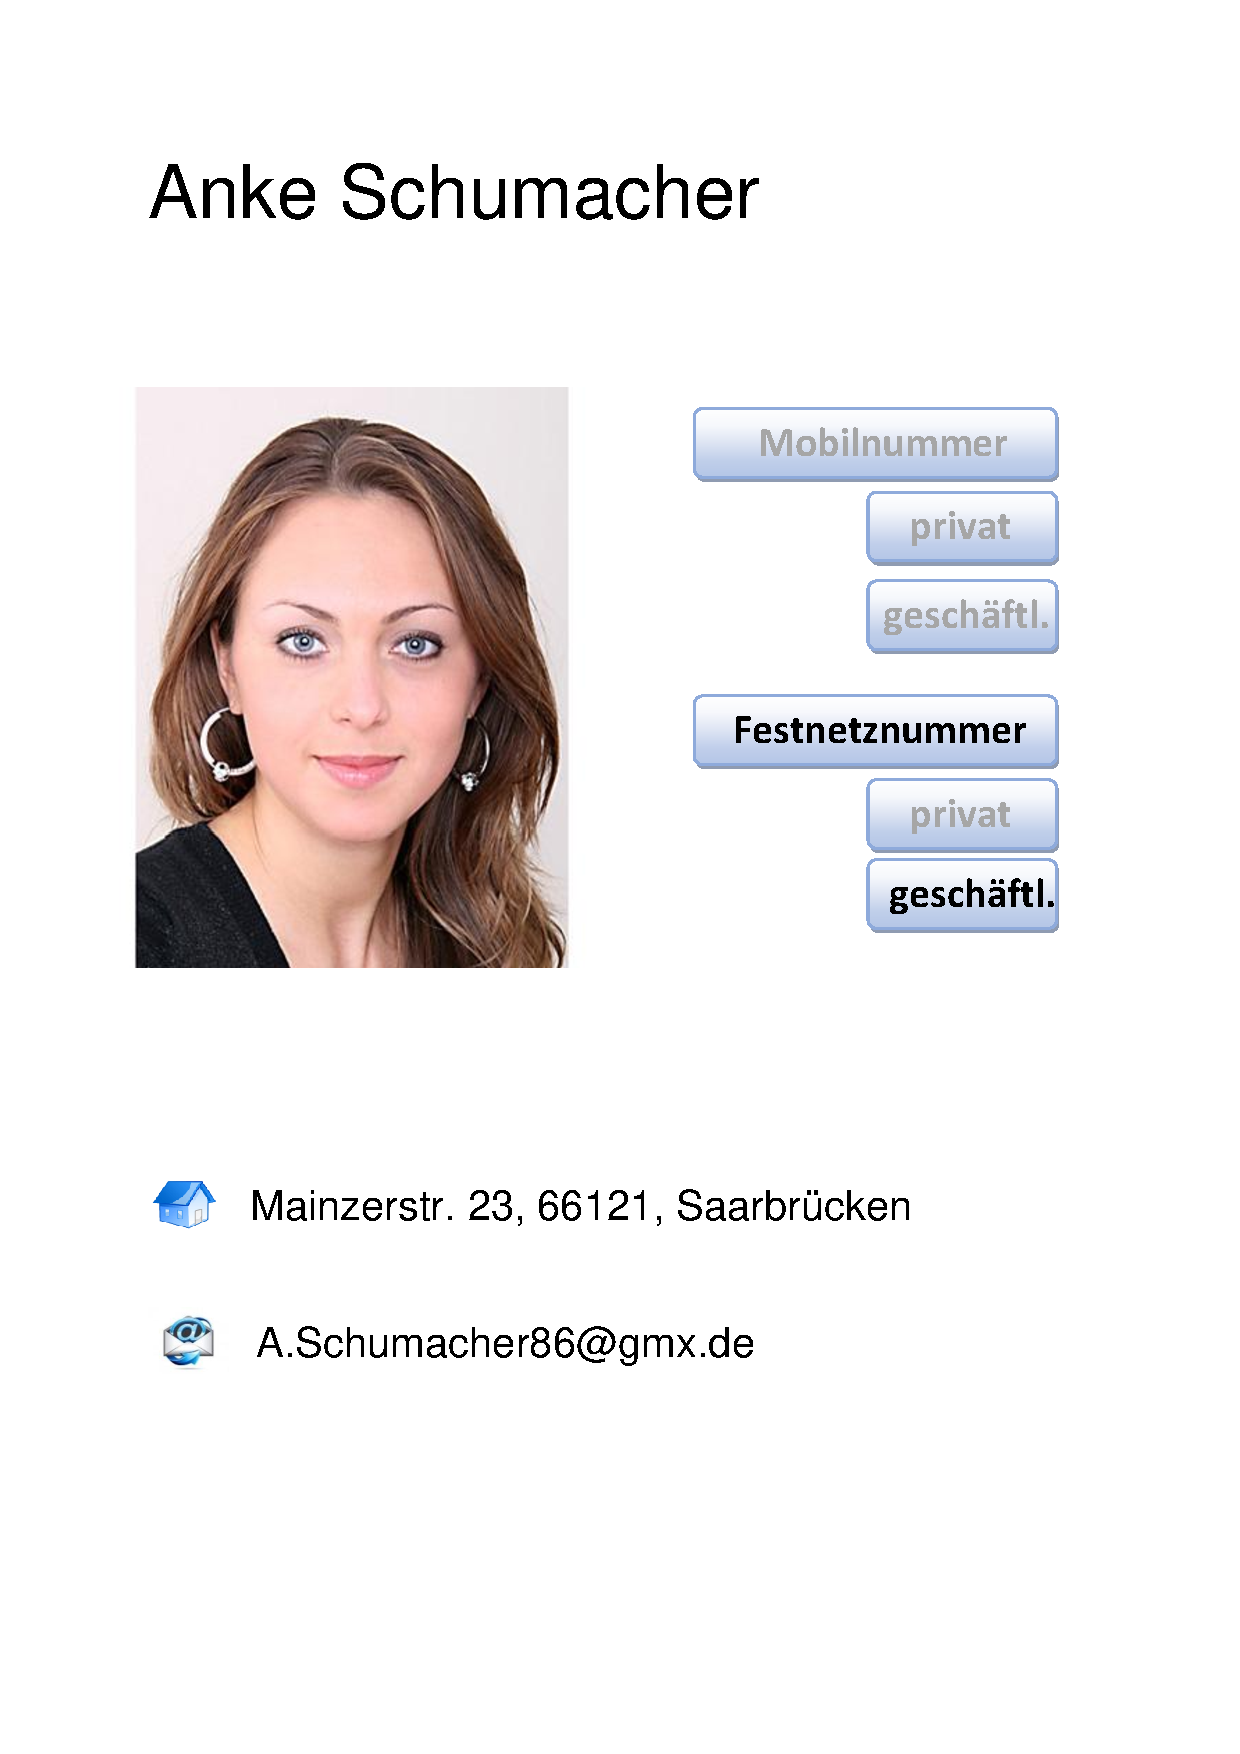
\includegraphics[width=12cm]{Anke.pdf}
\caption{Personenprofil: Anke im 1. Versuch}
\label{anke}
\end{center}
\end{figure}
Die Versuchspersonen werden am Anfang darauf hingewiesen, dass sie die Slots einzeln übergeben sollen. Nachdem der Benutzer per Sprachsteuerung spezifiziert hat, welche Person er anrufen möchte, fragt das System selbst die erforderlichen Slots ab. Diese Nachfrage wird für jeden der vier Anrufe in den unterschiedlichen Dialogstrategien realisiert. Pro Anruf gibt es insgesamt zwei zu füllende Slots, die mit derselben Disambiguierungsstrategie abgefragt werden. Der nächste Anruf unterscheidet sich in den zu füllenden Slots und der verwendeten Strategie. 
Die zu füllenden Slots sind in Tabelle \ref{slots} aufgelistet. Welche Slots pro anzurufenden Kontakt abgefragt werden, zeigt Tabelle \ref{slotsPerson}. Damit man später die Dialogzeiten für jede Strategie vergleichen kann, soll bei jedem Anruf der Slot an zweiter Stelle der Disambiguierung gefüllt werden. Wann die zu füllenden Slots abgefragt werden, wissen die Versuchspersonen jedoch nicht.  

\begin{longtable}{p{6cm}p{8cm}}
	\label{slots}\\
	\caption[Slotabfragen]{Beispiel Slotabfragen}\\
	\hline
	\textbf{Slot} &	\textbf{erfragte Werte}\\
	\hline
	\endfirsthead
	\hline
	\textbf{Slot} &	\textbf{erfragte Werte}\\
	\hline
	\endhead
Nummerntyp & Privat oder geschäftlich?\\
Telefontyp & Mobilnummer oder Festnetznummer\\
Nachname & Meier oder Müller\\
Stadt & München oder Ingolstadt\\


\hline
\end{longtable}


\begin{longtable}{p{3,2cm}p{3,2cm}p{3,2cm}p{3,2cm}}
	\label{slotsPerson}\\
	\caption[Slotabfrage pro Person]{Slotabfrage pro Person}\\
	\hline
	\textbf{Anke}&\textbf{Peter}&\textbf{Fritz} &\textbf{Kim}\\
	\hline
	\endfirsthead
	\hline
	\textbf{Anke}&\textbf{Peter}&\textbf{Fritz} &\textbf{Kim}\\
	\hline
	\endhead
Nummerntyp & & Nummerntyp & Nummerntyp\\
Telefontyp & Telefontyp & & Telefontyp \\
& Nachname & & \\
& & Stadt & \\

\hline
\end{longtable}


\subsection{Versuchsaufbau}
Um eine möglichst realistische Fahrsimulation mit hoher kognitiver Belastung darzustellen, werden die Versuchspersonen ein Rennspiel spielen. Durch die Nutzung eines extra für Rennspiele konzipierten Lenkrads, inklusive Gas- und Bremspedal, entsteht ein realitätsgetreues Fahrgefühl. Bei dem Rennspiel handelt es sich um \texttt{Need for Speed: Shift}, welches im Einzelrennen - Modus mit jeweils fünf Gegnern gefahren wird. Abbildung \ref{nfsss} zeigt einen Ausschnitt des Rennspiels während dem Versuch. 

\begin{figure}[H]
\begin{center}
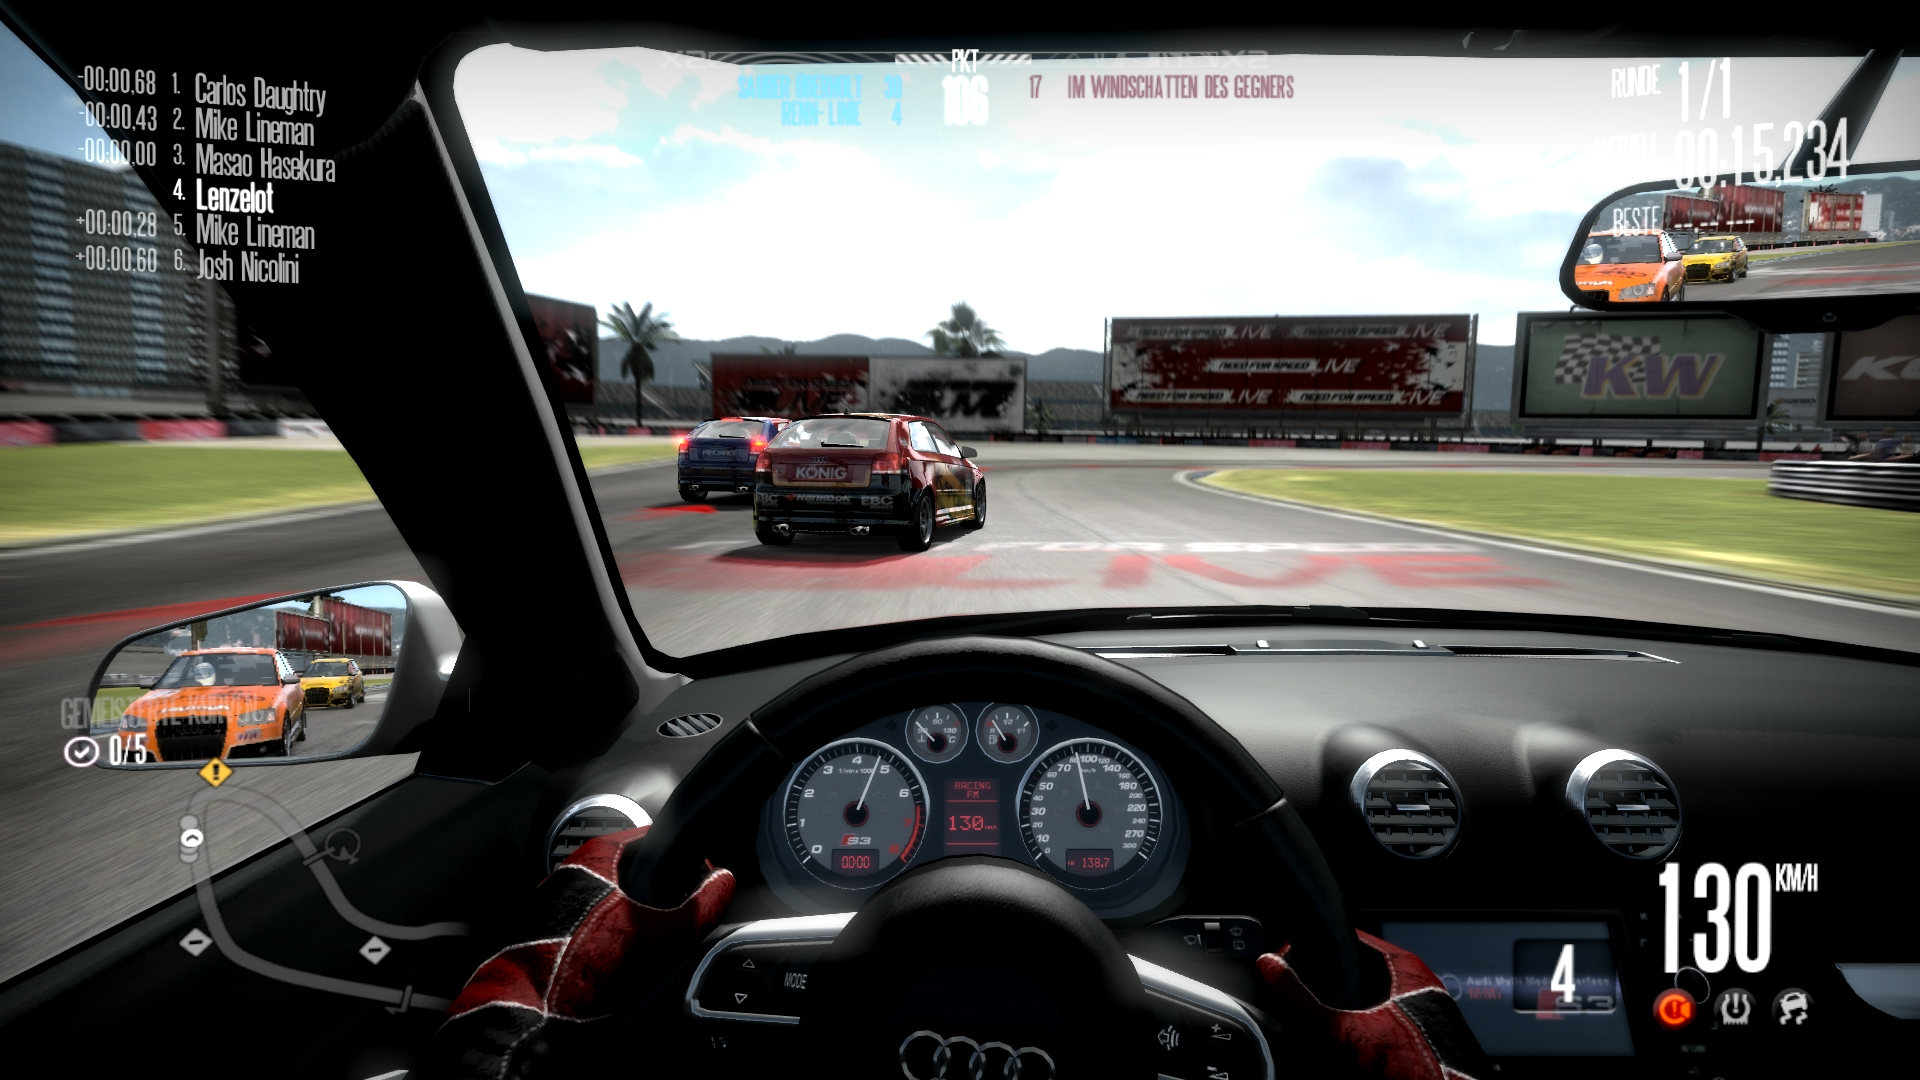
\includegraphics[width=14cm]{nfs.png}
\caption{Rennspiel während des Versuchs}
\label{nfsss}
\end{center}
\end{figure}

Die Versuchspersonen sollen neben der Interaktion mit dem Dialogsystem auch eine möglichst hohe Platzierung erreichen. Dies soll die Konzentration und damit die kognitive Belastung während dem Rennspiel steigern. Zu Beginn des Versuchs fahren die Probanden zunächst eine Testrunde. Das Ergebnis dieser Runde bietet eine Einschätzung darüber, wie schwer bzw. einfach das Rennspiel einer Testperson fiel. In den nächsten drei Runden werden die Versuchspersonen parallel zum Rennspiel das Testszenario durchgehen und dabei drei Personen anrufen. 

 Der Anruf gilt nur dann als erfolgreich, wenn alle Slots korrekt gefüllt werden. 
In der letzten Runde findet nur eine Systeminteraktion statt, ohne paralleles Rennspiel und die dadurch verursachte kognitive Belastung. 
Tabelle \ref{ablauf1} zeigt eine Übersicht des Versuchsaufbaus.

\begin{longtable}{p{2,4cm}p{2,4cm}p{2,4cm}p{2,4cm}p{2,4cm} }
	\label{ablauf1}\\
	\caption[Übersicht Versuchsablauf]{Übersicht Versuchsablauf}\\
	\hline
	\textbf{Vorrunde}&\textbf{1. Runde}&\textbf{2. Runde} &\textbf{3. Runde} & \textbf{4. Runde}\\
	\hline
	\endfirsthead
	\hline
	\textbf{Vorrunde}&\textbf{1. Runde}&\textbf{2. Runde} &\textbf{3. Runde} \textbf{4. Runde}\\
	\hline
	\endhead
Rennspiel & Rennspiel & Rennspiel & Rennspiel &\\
 & Anruf Anke & Anruf Peter & Anruf Fritz & Anruf Kim \\
\hline
\end{longtable}
Während des Versuchs werden die Versuchspersonen, das Rennspiel und die Dialoginteraktion aufgezeichnet. Dadurch wird sichergestellt, dass man alle Reaktionen einfangen und die Daten besser auswerten kann. 

\subsection{Versuchsdesign}
Die Versuchspersonen fahren in den Runden 1-3 jeweils eine Strecke mit unterschiedlicher Disambiguierungsstrategie. Insgesamt werden diese auf drei verschiedene Strecken verteilt, um einen Lerneffekt bei einer gleichbleibenden Strecke auszuschließen. Parallel  werden die Zeiten gemessen, die eine Versuchsperson für die Absolvierung einer Strecke bei der Interaktion mit einer bestimmten Disambiguierungsstrategie benötigt (siehe Unterkapitel \ref{messwerte1} Gemessene Zeiten). Da man diese Zeiten miteinander vergleichen möchte, müssen die Disambiguierungsstrategien geschickt auf die Strecken verteilt werden, da die Strecke unterschiedlich lang sind und daher keine aussagekräftigen Vergleiche untereinander bieten. Um diesen Konflikt zu lösen, werden die Versuchspersonen in drei Gruppen aufgeteilt, sodass jede Gruppe jede Strecke mit einer unterschiedlichen Disambiguierungsstrategie fährt. Schließlich kann man so für jede Strecke die Zeiten für unterschiedliche Strategien sammeln und vergleichen, mit welcher Strategie eine bestimmte Strecke am schnellsten gefahren wurde. \\
In der letzten Runde wird nur das Testszenario ohne Rennspiel durchgeführt. Hierfür gibt es Gruppe 4, welche aus allen Versuchsteilnehmern besteht. Diese wird jedoch nochmal in drei Zwischengruppen aufgeteilt, sodass ein Drittel der Versuchspersonen in der vierten Runde das Testszenario in Strategie 1, ein Drittel in Strategie 2 und das letzte Drittel in Strategie 3 durchführen. Ein Überblick der Strecken- und Strategieverteilung pro Gruppe ist in Tabelle \ref{verteilung1} aufgelistet. 

\begin{longtable}{p{3cm}p{3cm}p{3cm}p{3cm} }
	\label{verteilung1}\\
	\caption[Strecken- und Strategieverteilung]{Strecken- und Strategieverteilung}\\
	\hline
	\textbf{Aufteilung}&\textbf{Strategie 1}&\textbf{Strategie 2} &\textbf{Strategie 3}\\
	\hline
	\endfirsthead
	\hline
	\textbf{Aufteilung}&\textbf{Strategie 1}&\textbf{Strategie 2} &\textbf{Strategie 3}\\
	\hline
	\endhead
1. Gruppe & Strecke A & Strecke B & Strecke C \\
2. Gruppe & Strecke B & Strecke C & Strecke A \\
3. Gruppe  & Strecke C & Strecke A & Strecke B \\
4. Gruppe   & keine Strecke & keine Strecke & keine Strecke\\ 
\hline
\end{longtable}

Jede Gruppe fährt die Strecken in der gleichen Reihenfolge (erst Strecke A dann Strecke B und schließlich Strecke C). Dadurch wird gewährleistet, dass die Streckenzeiten durch keinen Lerneffekt bei einer unterschiedlichen Reihenfolge beeinflusst werden. Bei inkonsistenter Reihenfolge könnten die Resultate für die zuerst gefahrene Strecke aufgrund geringer Rennerfahrung schlechter ausfallen, als für die zuletzt gefahrene Strecke. Wenn Strecke A mal zu Beginn und mal zum Schluss gefahren wird, so könnten die Zeiten für die Runde am Schluss besser ausfallen, da die Versuchsperson durch die vorherigen Runden mehr an Spielerfahrung gewonnen hat und bessere Zeiten fährt. Die anzurufenden Personen sind auf bestimmte Strecken festgelegt und in Tabelle \ref{anrufstrecke1} gelistet. 

\begin{longtable}{p{6cm}p{6cm}}
	\label{anrufstrecke1}\\
	\caption[Anruf pro Strecke]{Anruf pro Strecke}\\
	\hline
	\textbf{Strecke} &	\textbf{Anruf}\\
	\hline
	\endfirsthead
	\hline
	\textbf{Strecke} &	\textbf{Anruf}\\
	\hline
	\endhead
Strecke A & Anke\\
Strecke B & Peter\\
Strecke C & Fritz\\
keine Strecke & Kim\\


\hline
\end{longtable}

\subsection{Control Panel}
\label{ControlPanel}
Um ein laufendes System zu simulieren wurde ein Control Panel entwickelt, welches verschiedene Sprachausgaben per Mausklick abspielen kann. Damit kann der Versuchsleiter die passenden Sprachausgaben auf entsprechende Benutzereingaben auslösen. Neben Ausgaben für die einzelnen Disambiguierungsstrategien sind weitere Sprachausgaben abgedeckt, welche oberflächlich zu jeder Eingabe des Benutzers eine Antwort bereitstellen und somit einen ungehinderten Ablauf des Dialogs gewährleisten. Zusätzlich dazu ist ein Stoppbutton enthalten, mit welchem per Klick alle aktiven Sprachausgaben abgebrochen werden können. 
\begin{comment}
Das Control Panel wurde mit JavaFx\footnote{\label{foot:javafx}\url{http://docs.oracle.com/javase/8/javase-clienttechnologies.htm}} entwickelt. Mit Hilfe des Programms JavaFX Scene Builder\footnote{\label{foot:fxsb}\url{http://www.oracle.com/technetwork/java/javase/downloads/javafxscenebuilder-info-2157684.html}} wurde zunächst das Design entwickelt. Anschließend wurden die Funktionen für die Sprachausgaben und des Stopp-Buttons implementiert. Die Sprachausgaben wurden online auf der Webseite \url{http://www.fromtexttospeech.com/} generiert. 
\end{comment}
Abbildung \ref{cp1} zeigt das Control Panel. Für jede anzurufende Person gibt es ein extra Tab mit personenspezifischen Sprachausgaben. Die gemeinsamen Sprachausgaben wie \texttt{Cancel} und der Stoppbutton sind in jedem Personen-Tab extra enthalten, damit eine schnelle Reaktion des Versuchsleiters möglich ist. Das Commons-Tab enthält die Begrüßungsausgabe. Zur Orientierung ist nach jedem spezifischen Button die ausgelöste Sprachausgabe zu sehen. 
\begin{figure}[htbp]
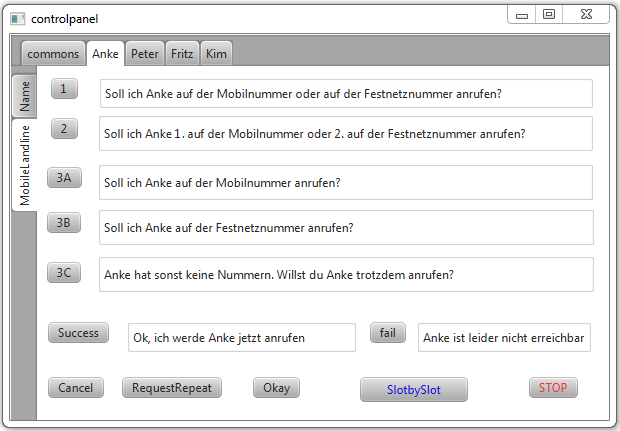
\includegraphics[width=13cm]{controlpanel.png}
\caption{Controlpanel Versuch 1}
\label{cp1}
\end{figure}

\subsection{Versuchspersonen}
Es wurden 12 deutsche Muttersprachler in einer Alterspanne von 18-53 Jahren getestet. Zu Beginn wurden die Versuchspersonen gleichmäßig aber zufällig einer Gruppe zugeteilt, durch die bestimmt wird, welche Strategie auf welcher Strecke gefahren wird (siehe Tabelle \ref{verteilung1}).
Der Versuchsablauf für die Versuchsperson sah folgendermaßen aus:
\begin{enumerate}
\item Testrunde fahren
\item Fragebogen über Person ausfüllen (siehe \ref{fbperson1} Unterkapitel Person)
\item Strecke A fahren + Anke anrufen
\item Fragebogen über kognitive Belastung und letzten Dialog ausfüllen (siehe \ref{fragebogen1} Unterkapitel Fragebogen)
\item Strecke B fahren + Peter anrufen
\item Fragebogen über kognitive Belastung und letzten Dialog ausfüllen
\item Strecke C fahren + Fritz anrufen
\item Fragebogen über kognitive Belastung und letzten Dialog ausfüllen 
\item Kim anrufen
\item Fragebogen über kognitive Belastung und letzten Dialog ausfüllen 
\end{enumerate}

Da den Versuchspersonen mitgeteilt wurde, dass sie mit einem echten System interagieren, sollten sie während des Dialogs deutlich in ein Tischmikrofon sprechen. Die Personenprofile konnten sie während des gesamten Dialoges über einen Laptop ansehen.

\subsection{Auswertung}
\label{auswertung1}
Um herauszufinden, welche Disambiguierungsstrategie am effizientesten ist, werden verschiedene Auswertungen vorgenommen. 
Zunächst werden die Zeiten gemessen, die die Versuchsperson zum einen für das absolvieren der Strecke und zum anderen für das erfolgreiche abschließen des Testszenarios benötigt (\ref{messwerte1} Gemessene Zeiten).
Außerdem werden die Fragebögen ausgewertet, die von den Versuchsperson nach jeder Runde ausgefüllt werden. Diese beziehen sich auf die subjektiv wahrgenommene kognitive Belastung und auf Merkmale der Disambiguierungsstrategien (\ref{fragebogen1} Fragebogen). Des Weiteren wird die Task Completion ausgewertet um zu erforschen, wie erfolgreich ein Dialog geführt wurde (\ref{tcausw1} Task Completion). Schließlich wird überprüft, wie die Versuchspersonen auf Rückfragen geantwortet haben und ob es dabei einen Unterschied zwischen hoch und niedrig belastenden Personen gibt (\ref{disverh1} Dialogverhalten). \\
Um die Aussagekraft der Ergebnisse zu ermitteln, wird zusätzlich die statistische Signifikanz mit Hilfe des Tukey-Test ermittelt. 
\subsubsection{Gemessene Zeiten}
\label{messwerte1}
\paragraph{Rennzeiten} 
~\\
%\textbf{Rennzeiten}\\
Um zu analysieren, ob das Rennverhalten durch eine Disambiguierungsstrategie negativ beeinflusst wird, werden die Rennzeiten pro Runde gemessen. Für jede Strecke wird die durchschnittliche Zeit gebildet, die die Versuchspersonen mit paralleler Systeminteraktion in einer bestimmten Strategie benötigten. Das Ergebnis ist in Tabelle \ref{RZ3SV1} aufgelistet.

\begin{longtable}{p{3cm}p{3cm}p{3cm}p{3cm} }
	\label{RZ3SV1}\\
	\caption[Durchschnittsrennzeiten jeder Strategie pro Strecke]{Durchschnittsrennzeiten jeder Strategie pro Strecke}\\
	\hline
	\textbf{Rennzeiten}&\textbf{Strategie 1}&\textbf{Strategie 2} &\textbf{Strategie 3}\\
	\hline
	\endfirsthead
	\hline
	\textbf{Rennzeiten}&\textbf{Strategie 1}&\textbf{Strategie 2} &\textbf{Strategie 3}\\
	\hline
	\endhead
Strecke A & 71,5 sek & 93 sek & 74,5 sek \\
Strecke B & 68,75 sek & 75,75 sek & 91,5 sek \\
Strecke C & 74,5 sek & 58,38 sek & 61,75 sek \\
\hline
\end{longtable}


Diesen Zeiten zufolge, wurde jede Strecke mit einer bestimmten Strategie am besten gefahren. Strecke A  und Strecke B wurde am schnellsten mit 71,5 Sekunden bzw. 68,75 Sekunden mit einer parallelen Dialoginteraktion in Strategie 1 gefahren. Mit Strategie 2 erfolgte die schnellste Rennzeit mit 58,38 Sekunden auf Strecke C. Diese Zeiten liegen jedoch nah beieinander und sind nicht aussagekräftig. Es gibt zudem keine Strategie, die durchweg auf allen Rennstrecken die besten Zeiten erzielen konnte. Dies könnte jedoch daran liegen, dass einzelnen Werte durch schlechtere bzw. bessere Spieler in den Gruppen verfälscht wurden.
Befindet sich zum Beispiel ein sehr schlechter Spieler in Gruppe 1 und ein sehr guter Spieler in Gruppe 2, so könnte die Durchschnittszeit für Strategie 1 auf Strecke A, durch die lange Zeit des schlechten Spielers, verschlechtert werden. Im Gegensatz dazu könnte die Durchschnittszeit für Strategie 3 auf Strecke A durch die guten Resultate des guten Spielers aus Gruppe 3 verbessert werden. Um dieses Problem zu lösen, wird pro Strategie der Durchschnitt aller mit dieser Strategie gefahrenen Rennzeiten berechnet. Zeiten von extrem guten bzw. schlechten Spielern sollten die Durchschnittszeiten ganzer Strategien dann nicht mehr beeinflussen. Die daraus resultierenden Werte geben dann eine Aussage darüber, mit welcher Strategie die Rennen am besten bzw. am schlechtesten gefahren wurden. 
Die endgültige Rennzeitberechnung für die Analyse der effizientesten Disambiguierungsstrategie ist in Tabelle \ref{RennZeitenDis1} dargestellt.

\begin{longtable}{p{3cm}p{3cm}p{3cm}p{3cm} }
	\label{RennZeitenDis1}\\
	\caption[Durchschnittsrennzeiten pro Strategie]{Durchschnittsrennzeiten pro Strategie}\\
	\hline
	\textbf{Rennzeiten}&\textbf{Strategie 1}&\textbf{Strategie 2} &\textbf{Strategie 3}\\
	\hline
	\endfirsthead
	\hline
	\textbf{Rennzeiten}&\textbf{Strategie 1}&\textbf{Strategie 2} &\textbf{Strategie 3}\\
	\hline
	\endhead
Durchschnitt & 71,58 sek & 75,71 sek & 75,92 sek\\
\hline
\end{longtable}
Die Unterschiede der Rennzeiten der einzelnen Strategien sind jedoch statistisch nicht signifikant. Daher kann hier nicht der Rückschluss gezogen werden, dass Strategie 1 wegen der insgesamt kürzesten Durchschnittsrennzeit die Versuchspersonen am wenigstens ablenkt. Des Weiteren bleibt die Frage offen, ob die Rennzeiten überhaupt Ausschluss darüber geben können, welche Strategie sich am besten während einer tatsächlichen Autofahrt eignet. Dies könnte in zukünftigen Arbeiten durch einen umfangreicheren Versuch überprüft werden. Möglicherweise könnten besser Ergebnisse erzielt werden, wenn die Rennstrecken kürzer gewählt werden. Im aktuellen Versuch dauert eine Rennstrecke im Durchschnitt circa 71 Sekunden und ein Dialog 19 Sekunden. Das heißt, dass hier nur ca. ein Viertel der Rennstrecke mit paralleler Systeminteraktion gefahren wird.


\begin{comment}
\begin{longtable}{p{3cm}p{3cm}p{3cm}p{3cm} }
	\label{durchschnittsvorl}\\
	\caption[Durschnittszeiten Strategie pro Strecke]{Durschnittszeiten Strategie pro Strecke}\\
	\hline
	\textbf{Rennzeiten}&\textbf{Strategie 1}&\textbf{Strategie 2} &\textbf{Strategie 3}\\
	\hline
	\endfirsthead
	\hline
	\textbf{Rennzeiten}&\textbf{Strategie 1}&\textbf{Strategie 2} &\textbf{Strategie 3}\\
	\hline
	\endhead
Strecke A & sek \O & sek \O & sek \O \\
Strecke B & sek \O & sek \O & sek \O\\
Strecke C  & sek \O & sek \O & sek \O\\

\hline
\end{longtable}


Tabelle \ref{durchschnittsvorl} ist nur eine Übergangstabelle, da  einzelnen Werte durch schlechte Spieler in den Gruppen verfälscht werden können. Befindet sich zum Beispiel ein sehr schlechter Spieler in Gruppe 1 und ein sehr guter Spieler in Gruppe 2, so könnte die Durschnittszeit für Strategie 1 auf Strecke A, durch die lange Zeit des schlechten Spielers, verschlechtert werden. Im Gegensatz dazu könnte die Durschnitsszeit für Strategie 3 auf Strecke A durch die guten Resultate von dem guten Spieler aus Gruppe 3 verbessert werden. Um dieses Problem zu lösen, nimmt man die Durchschnittszeiten aus Tabelle \ref{durchschnittsvorl} noch mal zum Durschnitt und erhält so eine Durschnittszeit pro Strategie. Die daraus resultierenden drei Werte sagen dann aus, mit welcher Strategie die Rennen am besten gefahren wurden. Zeiten von extrem guten bzw. schlechten Spielern sollten die Durschnittszeiten einzelner Strecken dann nicht mehr beeinflussen.  
Die endgültige Zeitberechnung für die Analyse der effizientesten Disambiguierungsstrategie ist in Tabelle \ref{ZeitenDis} dargestellt.
\end{comment}


\paragraph{Dialogzeiten}
~\\
Neben den Zeiten für das Rennspiel werden auch die Dialogzeiten gemessen. Anhand dieser Zeiten kann man sehen, mit welcher Strategie der kürzeste Dialog möglich ist. Des Weiteren kann man durch einen Vergleich der Dialogzeiten, die Unterschiede in der Effizienz der Strategie mit und ohne kognitive Belastung durch das Autorennen sehen. Das könnte interessant sein, um die Unterschiede im Dialogverhalten zwischen einer kognitiv hoch belastenden Versuchsperson und einer weniger belastenden Person zu untersuchen. Eine längere Dialogzeit in einer gleichen Strategie ist möglicherweise auf eine längere Reaktionszeit zurückzuführen, weshalb bessere Zeiten in der vierten Runde, also ohne Rennspiel und damit ohne hohe kognitive Belastung, erwartet werden. Es werden alle Dialogzeiten aus den Runden mit Rennspiel gemessen. Aus diesen Zeiten lässt sich dann pro Strecke ein Durchschnittswert bilden. Neben diesen Werten wird zudem die gesamte durchschnittliche Dialogzeit pro Strategie gebildet. Diese Werte kann man mit den Durchschnittszeiten aus der Runde ohne Rennstrecke vergleichen. Es werden allerdings nur die Dialogzeiten bewertet, die einen korrekt durchgeführten Dialog abbilden um die Durchschnittszeiten nicht zu verfälschen.  Tabelle \ref{Durchschnittsdialogzeiten1} zeigt diese Ergebnisse.

\begin{longtable}{p{3cm}p{3cm}p{3cm}p{3cm} }
	\label{Durchschnittsdialogzeiten1}\\
	\caption[Durchschnittsdialogzeiten]{Durchschnittsdialogzeiten}\\
	\hline
	\textbf{Dialogzeiten}&\textbf{Strategie 1}&\textbf{Strategie 2} &\textbf{Strategie 3}\\
	\hline
	\endfirsthead
	\hline
	\textbf{Rennzeiten}&\textbf{Strategie 1}&\textbf{Strategie 2} &\textbf{Strategie 3}\\
	\hline
	\endhead
Strecke A & 15,34 sek & 20,38 sek & 20,28 sek \\
Strecke B & 14,31 sek & 20,05 sek & 22,07 sek \\
Strecke C  & 15,97 sek & 21,01 sek & 20,35 sek \\
\hline
\hline
Strecke A - C & 15,19 sek & 20,52 sek & 20,81 sek \\
\hline
ohne Strecke &  14,9 sek & 18,8 sek & 17,59 sek \\
\hline
\end{longtable}

Die Unterschiede in den Dialogzeiten zwischen Strategie 1 und Strategie 2, sowie zwischen Strategie 1 und Strategie 3 sind statistisch signifikant. Die Unterschiede der Zeiten zwischen Strategie 2 und Strategie 3 sind nicht signifikant. Das Ergebnis zeigt, dass die Strategie 1 den kürzesten Dialog sowohl mit Rennspiel, als auch ohne Rennspiel ermöglicht. Die letzten beiden Zeilen der Tabelle zeigen, dass die Versuchspersonen einen kürzeren Dialog in jeder Strategie ohne Rennspiel ablegen. Die Ergebnisse aus \ref{disverh1} (Dialogverhalten) lassen ausschließen, dass die Unterschiede aufgrund unterschiedlichen Dialogverhaltens zustande kommen. Dies lässt vermuten, dass die Reaktionszeiten bei geringer Belastung schneller sind als bei hoher Belastung und die zeitlichen Unterschiede dadurch zu Stande kommen. 
\subsubsection{Fragebogen}
\label{fragebogen1}
Neben den Zeiten wird der Fragebogen jeder Runde ausgewertet. Dieser besteht im ersten Teil aus einem Ausschnitt des NASA-TLX Testes zur subjektiven Einschätzung der empfundenen kognitiven Belastung\footnote{\label{foot:nasatlx1}\url{http://www.keithv.com/software/nasatlx/nasatlx_german.html}} . Im zweiten Teil werden Fragen über die zuletzt verwendete Dialogstrategie gestellt und es wird die Möglichkeit gegeben positives oder negatives Feedback über den Dialog der letzten Runde zu geben. Zu Beginn des Versuchs wird ein allgemeiner Fragebogen ausgefüllt, der Informationen zur Versuchsperson liefert. 
\paragraph{Nasa-TLX}
~\\
Abbildung \ref{fbnasatlx1} zeigt den NASA-TLX Fragebogen. 
Die Ergebnisse dieses Testes werden zum einen dafür genutzt um zu erforschen, bei welcher Strategie die Versuchspersonen eine höhere kognitive Belastung empfunden haben. Zum anderen kann man sehen, wie die Versuchspersonen ihre kognitive Belastung während einer Runde mit Rennspiel im Vergleich zur Runde ohne Rennspiel einschätzen. 

\begin{figure}[H]
\begin{center}
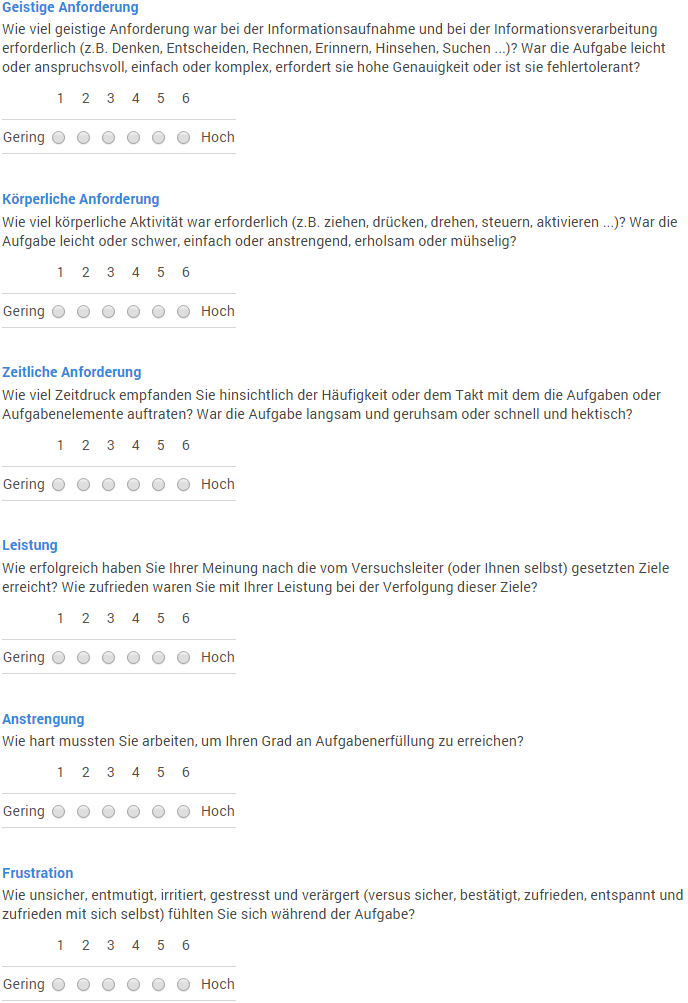
\includegraphics[width=12cm]{nasa.png}
\caption{Fragebogen: NASA-TLX}
\label{fbnasatlx1}
\end{center}
\end{figure}

Die nachfolgende Tabelle zeigt die Ergebnisse des Fragebogens. Dabei werden jeweils die durchschnittlichen Antworten für alle Runden (1-4), der Runden mit Rennspiel (1-3) und der Runde ohne Rennspiel (4) aufgelistet und für jede Strategie einzeln gewertet. \newpage


\begin{longtable}{|p{4cm}|p{2cm}|p{2cm}|p{2cm}|p{2cm}|}
	\hline
		\textbf{Antwortenintervall}&\textbf{Strategien}&\multicolumn{3}{c|}{\textbf{Ergebnisse bestimmter Runden}}\\
	&&\textbf{1-4}&\textbf{1-3} &\textbf{4}\\
	\hline
	\endfirsthead
	\hline
	\textbf{Antwortenintervall}&\textbf{Strategien}&\textbf{Runden 1-4}&\textbf{Runden 1-3} &\textbf{Runde 4}\\
	\hline
	\endhead
		\multicolumn{5}{l}{\textbf{Geistige Anforderung}}\\
		\hline
\multirow{3}{4cm}{1: gering \newline 6: hoch} & Strategie 1 &  1,88 & 2,08 & 1,25 \\
 & Strategie 2 & 2,06 & 2,42 & 1\\
 & Strategie 3 & 2,63 & 2,83 & 2 \\
\hline
		\multicolumn{5}{l}{\textbf{Körperliche Anforderung}}\\
		\hline
\multirow{3}{4cm}{1: gering \newline 6: hoch} & Strategie 1 & 2 & 2,17 & 1,5 \\
 & Strategie 2 & 1,44 & 2,25 & 1 \\
 & Strategie 3 & 2 & 2,25 & 1,25 \\
\hline
		\multicolumn{5}{l}{\textbf{Zeitliche Anforderung}}\\
		\hline
\multirow{3}{4cm}{1: gering \newline 6: hoch} & Strategie 1 & 1,87 & 2,09 & 1,25 \\
 & Strategie 2 & 1,75 & 2 & 1 \\
 & Strategie 3 & 2,31 & 2,67 & 1,25 \\
\hline
		\multicolumn{5}{l}{\textbf{Leistung}}\\
		\hline
\multirow{3}{4cm}{1: gering \newline 6: hoch} & Strategie 1 & 4,25 & 4,5 & 3,5 \\
 & Strategie 2 & 4,75 & 4,33 & 6 \\
 & Strategie 3 & 4,25 & 4 & 5 \\
\hline
		\multicolumn{5}{l}{\textbf{Anstrengung}}\\
		\hline
\multirow{3}{4cm}{1: gering \newline 6: hoch} & Strategie 1 & 2 & 2,25 & 1,25 \\
 & Strategie 2 & 2,13 & 2,55 & 1 \\
 & Strategie 3 & 2,63 & 2,92 & 1,75\\
\hline
		\multicolumn{5}{l}{\textbf{Frustration}}\\
		\hline
\multirow{3}{4cm}{1: gering \newline 6: hoch} & Strategie 1 & 1,69 & 1,83 & 1,25 \\
 & Strategie 2 & 1,81 & 2,08 & 1 \\
 & Strategie 3 & 2 & 2,25 & 1,25 \\
\hline
\end{longtable}

Die Unterschiede der Antworten einzelner Strategien sind nicht signifikant, sodass nicht eindeutig gesagt werden kann, welche Strategie die Versuchsperson am meisten bzw. am wenigsten belastet. Betrachtet man jedoch die Ergebnisse aller Fragen fällt auf, dass die Antworten im Bezug auf geistige Anforderung, die Anstrengung und die Frustration zeigen, dass die erste Strategie als am wenigsten belastend und die dritte Strategie als am belastendsten empfunden wurde. Dies deckt sich auch mit den Ergebnissen aus dem zweiten Teil des Fragebogens, in welchem die erste Strategie als Favorit und die dritte Strategie als unbeliebteste Strategie gewertet wurde. \newline \newline Vergleicht man die Werte für Runde 1-3 mit den Werten von Runde 4 fällt auf, dass die Dialoge parallel zum Rennspiel durchweg, mit Ausnahme der Frage nach der Leistung, als belastender gewertet wurden als die Dialoge ohne Rennspiel. Dies zeigt, dass die Versuchspersonen einen Unterschied in der kognitiven Belastung gespürt haben.   
\paragraph{Strategien}
~\\
Der zweite Teil des Fragebogens ist in Abbildung \ref{fbstrategien1} zu sehen. 
Mit diesem Fragebogen werden die einzelnen Strategien anhand verschiedener Kategorien bewertet.
\begin{figure}[H]
\begin{center}
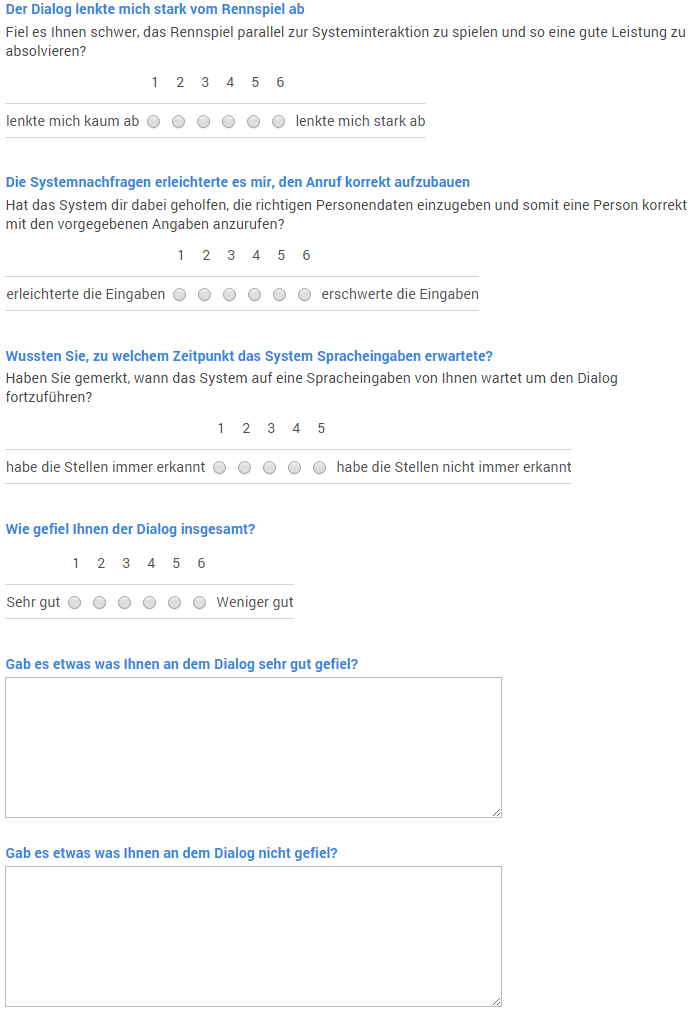
\includegraphics[width=12cm]{fbdialog.png}
\caption{Fragebogen: Dialogstrategien}
\label{fbstrategien1}
\end{center}
\end{figure}
Die nachfolgende Tabelle zeigt die Ergebnisse des Fragebogens. Dabei werden jeweils die durchschnittlichen Antworten für alle Runden (1-4), der Runden mit Rennspiel (1-3) und der Runde ohne Rennspiel (4) aufgelistet und für jede Strategie einzeln gewertet.
\newline \newline
Da die Interaktion mit dem Dialogsystem in Runde 4 ohne Rennspiel erfolgt, wird die Frage \texttt{"Der Dialog lenkte mich vom Rennspiel ab"} für diese Runde nicht beantwortet. Entsprechend wird die Frage \texttt{"Fiel es Ihnen einfacher, den Dialog ohne Rennspiel zu führen?"} nur für die 4. Runde beantwortet.
Die Frage \texttt{"Welcher Anruf gefiel Ihnen insgesamt am besten?"} wird zum Schluss beantwortet.
\newpage

\begin{longtable}{|p{4cm}|p{2cm}|p{2cm}|p{2cm}|p{2cm}|}
	\hline
		\textbf{Antwortenintervall}&\textbf{Strategien}&\multicolumn{3}{c|}{\textbf{Ergebnisse bestimmter Runden}}\\
	&&\textbf{1-4}&\textbf{1-3} &\textbf{4}\\
	\hline
	\endfirsthead
	\hline
	\textbf{Antwortenintervall}&\textbf{Strategien}&\textbf{Runden 1-4}&\textbf{Runden 1-3} &\textbf{Runde 4}\\
	\hline
	\endhead
		\multicolumn{5}{l}{\textbf{Der Dialog lenkte mich vom Rennspiel ab}}\\
		\hline
\multirow{3}{4cm}{1: kaum \newline 6: stark} & Strategie 1 & - & 2,25  & - \\
 & Strategie 2 & - & 2,58 & - \\
 & Strategie 3 & - & 2,58 & -\\
\hline
		\multicolumn{5}{l}{\textbf{Die Nachfragen erleichterten es mir, den Anruf korrekt aufzubauen}}\\
		\hline
\multirow{3}{4cm}{1: erleichterte es\newline  6: erschwerte es} & Strategie 1 & 1,63 & 1,83 & 1,25 \\
 & Strategie 2 & 1,69 & 1,92 & 1 \\
 & Strategie 3 & 2,13 & 2,25 & 1,75 \\
\hline
		\multicolumn{5}{l}{\textbf{Wussten Sie, wann das System Spracheingaben erwartete?}}\\
		\hline
\multirow{3}{4cm}{1: immer \newline  6: nicht immer} & Strategie 1 & 1,19 & 1,17 & 1,25 \\
 & Strategie 2 & 1,38 & 1,33 & 1,5 \\
 & Strategie 3 & 1,5 & 1,67 & 1 \\
\hline
		\multicolumn{5}{l}{\textbf{Wie gefiel Ihnen der Dialog insgesamt?}}\\
		\hline
\multirow{3}{4cm}{1: sehr gut \newline  6: weniger gut} & Strategie 1 & 1,94 & 2,08 & 1,5 \\
 & Strategie 2 & 2,50 & 2,67 & 2 \\
 & Strategie 3 & 2,57 & 2,75 & 2 \\
\hline
		\multicolumn{5}{l}{\textbf{Fiel es Ihnen einfacher, den Dialog ohne Rennspiel zu führen?}}\\
		\hline
\multirow{3}{4cm}{1: viel einfacher \newline  6: nicht einfacher} & Strategie 1 &  - & - & 2 \\
 & Strategie 2 & - & - & 3,75 \\
 & Strategie 3 & - & - & 2,25\\
\hline
		\multicolumn{5}{l}{\textbf{Welcher Anruf gefiel Ihnen insgesamt am besten?}}\\
		\hline
\multirow{3}{4cm}{Anruf bzw. Strategie auswählbar} & Strategie 1 & 75\% & - & - \\
 & Strategie 2 & 16,6\% & - & - \\
 & Strategie 3 & 8,3\% & - & - \\
\hline
\end{longtable}

Die ersten vier Antworten dieses Fragebogens zeigen, dass die erste Strategie am Positivsten und die dritte Strategie am Negativsten gewertet wurde. Dies stimmt mit dem Ergebnis der letzten Frage überein, welche konkret nach der beliebtesten Strategie fragt. \newline \newline Die vorletzte Frage zeigt, dass es dem Durchschnitt der Versuchspersonen einfacher fiel, den Dialog ohne Rennspiel zu führen. Dies bestätigt das Ergebnis aus dem NASA-TLX Fragebogen, welches besagt, dass die Versuchspersonen einen Unterschied in der kognitiven Belastung zwischen Dialog mit Rennspiel und ohne Rennspiel gemerkt haben.  

\paragraph{Person}
\label{fbperson1}
~\\
In Abbildung \ref{fbperson} sind die Fragen dieses Fragebogens abgebildet. Dieser Fragebogen dient dazu, um Informationen über die Versuchsperson zu erhalten.
Die Fragen nach der Rennspiel- und Dialogerfahrung können für die spätere Auswertung der Zeiten interessant sein und eine mögliche Erklärung für stark abweichende Rennspiel- und Dialogzeiten liefern. \newline \newline
Jeder Person wird eine ID zugeteilt. Diese wird zu Beginn jedes Fragebogens eingetragen, damit jeder Versuchsperson alle abgegebenen Antworten zugeordnet werden können. 

\begin{figure}[H]
\begin{center}
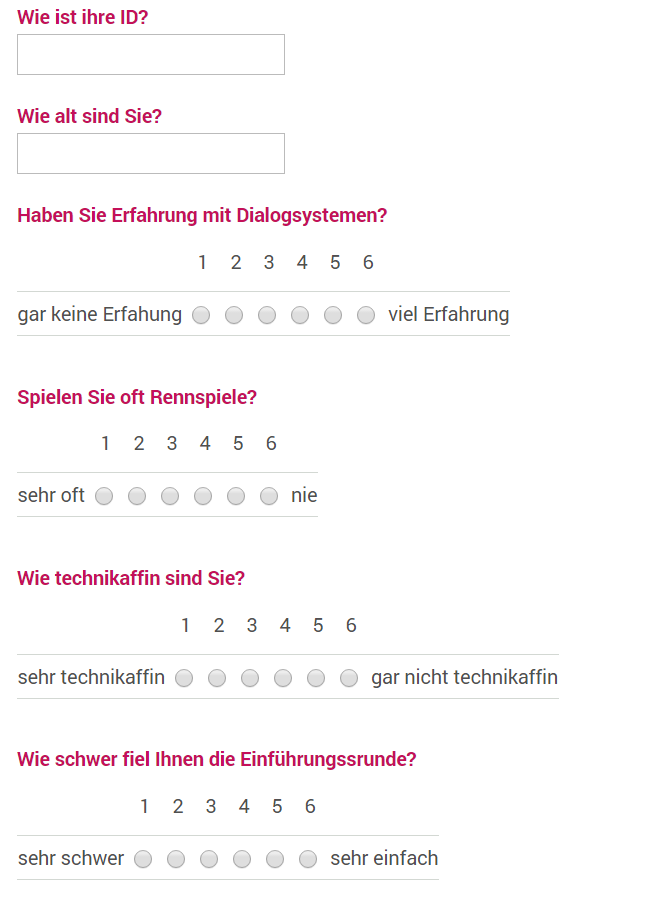
\includegraphics[width=12cm]{fbperson.png}
\caption{Fragebogen: Person}
\label{fbperson}
\end{center}
\end{figure}
\newpage


58\% der Probanten sind in einer Altersgruppe von 18-29, 17 \% in einer Altersgruppe von 30-41 und 25\% in einer Altersgruppe von 42-53. Alle Versuchspersonen sind deutsche Muttersprachler. 
Eine Zusammenfassung der restlichen Antworten steht in Abbildung \ref{fbpersonaus}.


\begin{figure}[H]
\begin{center}
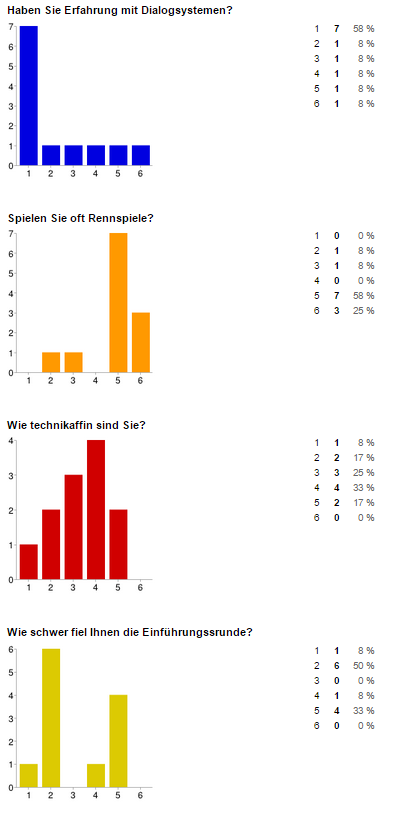
\includegraphics[width=10cm]{person1.png}
\caption{Fragebogen: Person}
\label{fbpersonaus}
\end{center}
\end{figure}
\newpage

Das Ergebnis zeigt, dass 75\% der Testpersonen keine bzw. wenig Erfahrung mit Dialogsystemen haben. Aus den Antworten lässt sich weiter schließen, dass 83\% der Befragten selten Rennspiele spielen und die Einführungsrunde 58\% schwer fiel. Daraus wird klar, dass die Mehrheit der Versuchspersonen unerfahren im Umgang mit Dialogsystemen und Rennspielen ist. In einer zukünftigen Arbeit könnte untersucht werden, ob das Ergebnisse des Versuchs abhängig von der Erfahrung der Versuchspersonen mit Dialogsystemen und Rennspielen ist. Dazu könnten die Testpersonen je nach Erfahrung in zwei Gruppen aufgeteilt und die Resultate miteinander vergleichen werden. 

\begin{comment}
\begin{longtable}{|p{4cm}|p{4cm}|p{4cm}|}
	\hline
	\textbf{Antwortenintervall}&\textbf{Antwort}&\textbf{Antworten in \%}\\
	\hline
	\endhead
		\multicolumn{3}{l}{\textbf{Wie alt sind Sie}}\\
		\hline
 & 18-29 &  58 \\
 & 30-41 &  17 \\
 & 41-53 &  25\\
\hline
		\multicolumn{3}{l}{\textbf{Haben Sie Erfahrung mit Dialogsystemen}}\\
		\hline
\multirow{2}{4cm}{1: gar keine \newline  6: viel } & 1-3 &  58 \\
 & 4-6 &  17 \\

\hline
		\multicolumn{3}{l}{\textbf{Spielen Sie oft Rennspiele}}\\
		\hline
\multirow{2}{4cm}{1: sehr oft \newline  6: nie } & 1-3 &  58 \\
 & 4-6 &  17 \\

\hline
		\multicolumn{3}{l}{\textbf{Wie technikaffin sind Sie}}\\
		\hline
\multirow{2}{4cm}{1: sehr \newline  6: gar nicht} & 1-3 &  58 \\
 & 4-6 &  17 \\

\hline
		\multicolumn{3}{l}{\textbf{Wie schwer fiel Ihnen die Einführungsrunde}}\\
		\hline
\multirow{2}{4cm}{1: sehr schwer\newline  6: sehr einfach} & 1-3 &  58 \\
 & 4-6 &  17 \\

\hline
\end{longtable}
\end{comment}


\subsubsection{Task Completion}
\label{tcausw1}
Für jede Strategie wird die Task Completion ausgewertet, welche besagt, mit welchem Erfolg das Testszenario ausgeführt wurde. Sie wird bemessen, in dem man für jeden richtig gefüllten Slot (siehe Tabelle \ref{slotsPerson}) einen Punkt verteilt. Folgenden Punktzahlen sind also für jede Strategie möglich:
\begin{itemize}
\item 0 Punkte, wenn kein Slot richtig gefüllt wird
\item 1 Punkt, wenn ein Slot richtig gefüllt wird
\item 2 Punkte, wenn alle Slots richtig gefüllt werden
\end{itemize}
Zur Auswertung wird pro Strategie eine Durchschnittspunktzahl berechnet. Die Durchschnittspunktzahlen für alle Runden (1-4), der Runden mit Rennspiel (1-3) und der Runde ohne Rennspiel (4) finden sich in Tabelle \ref{TCV1}.
\newpage

\begin{longtable}{p{3cm}p{3cm}p{3cm}p{3cm} }
	\label{TCV1}\\
	\caption[Durchschnittliche Task Completion pro Strategie]{Durchschnittliche Task Completion pro Strategie}\\
	\hline
\textbf{Strategien}&\textbf{insgesamt}&\textbf{Runde 1-3} &\textbf{Runde 4}\\
	\hline
	\endfirsthead
	\hline
	\textbf{Strategien}&\textbf{\O TC insgesamt}&\textbf{\O TC Runde 1-3} &\textbf{\O TC Runde 4}\\
	\hline
	\endhead
1. Strategie & 1,75 & 1,92 & 1,5  \\
2. Strategie & 1,94 & 1,92 & 2  \\
3. Strategie & 1,63 & 1,5 & 2  \\
\hline
Insgesamt & & 1,78 & 1,83 \\ 
\hline
\end{longtable}

Im Durchschnitt wurde in Runde 4 eine höhere Task Completion erreicht. Das besagt, dass die Dialoge der vierten Runde am erfolgreichsten durchgeführt wurden. Der Unterschied ist jedoch sehr gering, sodass man für ein eindeutiges Resultat mehr Ergebnisse zur Auswertung benötigt. Die Durchschnittspunktzahlen zeigen weiter, dass die zweite Strategie insgesamt am erfolgreichsten abgeschlossen wurde. Die erfolgloseste Strategie ist nach diesem Ergebnis die dritte Strategie. Dies passt zum Ergebnis, dass diese Dialogstrategie im Fragebogen über die Strategien (vgl. \ref{fragebogen1} Unterkapitel Strategien) am schlechtesten gewertet wurde. Strategie 1, welche als beliebteste Strategie der Runde 1-3 ausgewählt wurde, liefert für diese Runden die gleiche Task Completion wie Strategie 2. Hier fehlen weitere Ergebnisse um eine konkrete Verbindung zwischen beliebteste Strategie und Strategie mit höchster Task Completion herzustellen. Dabei muss auch der Fall betrachtet werden, dass die Versuchsperson ihre Fehler möglicherweise gar nicht bemerken. Diese Verbindung könnte in einem umfangreichen Experiment in späteren Arbeiten überprüft werden. 
Grundsätzlich kann man an diesem Ergebnis sehen, dass insgesamt der Anruf am häufigsten korrekt mit Strategie 2 und am seltensten korrekt mit Strategie 3 ausgeführt werden konnte. \newline
Es ist jedoch fraglich, ob die hier entstandenen Fehler auch in einem realen Dialog aufkommen, bei dem die Versuchsperson die Anrufattribute selbst bestimmt. Deshalb gibt diese Auswertung nur ein Indiz darauf, welche Strategie möglicherweise am kompliziertesten ist. 


\subsubsection{Dialogverhalten}
\label{disverh1}
Für jede Strategie werden die Antworten der Versuchspersonen gesammelt um festzustellen, ob es Unterschiede im Dialogverhalten unter hoher und niedriger kognitiver Belastung gibt. Alle gegebenen Antwortmöglichkeiten werden kurz erläutert und sind in Tabelle \ref{Dialogverhalten11} mit einem Beispiel aufgelistet.

\begin{description}
\item[Slots:] der zu füllende Slot wird als Antwort übergeben.
\item[Position:] es wird mit der Position des gewünschten Slotfüllers geantwortet.
\item[ja/nein:] der vorgeschlagenen Slotfüller wird angenommen bzw. abgelehnt.
\end{description}

\begin{longtable}{p{3,5cm}p{5cm}p{3,5cm}}
	\label{Dialogverhalten11}\\
	\caption[Antwortmöglichkeiten1]{Antwortmöglichkeiten}\\
	\hline
\textbf{Antwort-möglichkeiten}&\textbf{Beispiel \newline Slotabfrage}&\textbf{Beispiel \newline Antwort}\\
	%\hline
	%\endfirsthead
	%\hline
	%\textbf{Antwort-möglichkeiten}&\textbf{Beispiel \newline Slotabfrage}&\textbf{Beispiel \newline Antwort}\\
	\hline
	%\endhead
Slots  & Willst du Anke privat oder geschäftlich anrufen? & geschäftlich  \\
Position & Willst du Anke 1. privat oder 2. geschäftlich anrufen? & zweitens  \\
ja/nein & Willst du Anke privat anrufen? &  nein\\ 
\hline
\end{longtable}

Die Häufigkeiten dieser Antworten pro Strategie aus Runde 1-3 sind in nachfolgender Tabelle aufgelistet.

\begin{longtable}{p{3cm}p{3cm}p{3cm}p{3cm} }
	\label{Dialogverhalten12}\\
	\caption[Antwortenverteilung pro Strategie]{Antwortenverteilung pro Strategie}\\
	\hline
\textbf{Antwort-möglichkeiten}&\textbf{Strategie 1}&\textbf{Strategie 2} &\textbf{Strategie 3}\\
	\hline
	\endfirsthead
	\hline
	\textbf{Antwortmöglichkeiten}&\textbf{Strategie 1}&\textbf{Strategie 2} &\textbf{Strategie 3}\\
	\hline
	\endhead
Slots & 100\% & 70,8\%\ & 16,7\%  \\
Position & 0\% & 29,2\% & 0\%  \\
ja/nein & 0\% & 0\%  & 83,3 \%  \\
\hline
\end{longtable}

Um zu erforschen, ob sich das Dialogverhalten in Runde 4 ändert, wurden pro Person die Antworten aus der Strategie der 4. Runde mit der entsprechenden Strategie aus den Runden davor verglichen. Es hat sich herausgestellt, dass die Verteilung der Antwortmöglichkeiten bei hoher Belastung die gleiche ist wie bei niedriger Belastung.
 Dadurch ist kein Unterschied im Dialogverhalten bei unterschiedlicher Belastung erkennbar. 

\begin{comment}
\subsection{Hypothesen}
\textbf{beliebt}: kurze Sprachausgabe, kurze Spracheingabe, wenig Aufmerksamkeit \\
\textbf{unbeliebt}: lange Sprachausgaben mit unnötigen Informationen, anstrengendes Zuhören\\
\textbf{hoher CL}: kurze knappe Eingabe (BargeIn, Füllwörter), Confirmations bevorzugt (Related Work) und möglichst viele Pausen (Strat 3)\\
\textbf{kein/niedriger CL}: weniger BargeIn und Füllwörter(Related Work)


\subsection{Simulation und Durchführung}
Versuchspersonen bekommen bestimmte Aufgabe\\
\\
\texttt{Ich habe eine System für das Auto gebaut, mit welchem ihr Telefonieren könnt. Bitte testet mal alle Funktionen des Systems}\\
\\
$\rightarrow$ denken sie haben andere Aufgabe und wissen nicht was eigentlich getestet werden soll.\\
\\
Versuchspersonen sollen also pro Runde einen Kontakt anrufen\\
Dauer einer Runde je nach Können ca. 2-3 Minuten\\
?? Versuchspersonen können/sollen sich vor jeder Runde kurz durchlesen, welche Interaktionen möglich sind\\
Bei jeder Interaktion gibt es Stellen, an denen ambige Spracheingabe getriggert werden.
\\
Beispiele mit ambiger Satzeingabe und anschließender Disambiguierungsstrategie pro Aktion:
\\
\\
\texttt{1. Strategie}:\\
U: Rufe Paul an\\
S: Willst du Paul auf der Festnetznummer oder auf der Handynummer anrufen?\\
U: auf der Handynummer\\
\texttt{2. Strategie mit Barge-in}\\
U: Rufe Paul an\\
S: Willst du Paul auf 1. der Festnetznummer oder [..]  anrufen.\\
U: Ja\\
\texttt{2. Strategie mit deictit reference}\\
U: Rufe Paul an\\
S: Willst du Paul auf 1. der Festnetznummer oder 2. auf der\\ Handynummer anrufen.\\
U: ersteres
\texttt{3.Strategie}:\\
U: Rufe Paul an\\
S: Willst du Paul auf der Festnetznummer anrufen?\\
U: Nein\\
S: Willst du Paul auf der Handynummer anrufen?\\
U: ja
\\
\\
Die zu testenden Disambiguierungsstrategien sind über die Runden verteilbar.\\
Jede Versuchsperson bekommt alle Disambiguierungsstrategien während des Testen präsentiert.\\
Am Schluß des gesamten Test soll die Versuchsperson einen Fragebogen ausfüllen (Nasa TLX (related work))
\begin{itemize}
\item Wie intuitiv war die Interaktion zu führen
\item war die Interaktion während dem Fahren eher ablenkend oder störend?
\item wie viel Aufmerksamkeit musste man dem System während der Interaktion schenken
\item siehe nasa-tlx screenshot
\end{itemize}
??Anschließend über Disambiguierungsstrategien aufklären und über einzelne Strategien befragen.
?$\rightarrow$ welche Strategie war am geeignetsten/einfachsten/intuitivsten für jeweilige Versuchsperson

\end{comment}


\subsection{Resultat}
Aus den Resultaten aus Kapitel \ref{auswertung1} (Auswertung) wird die effizienteste Strategie ermittelt. \newline

Die Ergebnisse aus den Rennzeiten zeigen, dass die Rennstrecken mit Strategie 1 am Schnellsten befahren wurden. Dieses Resultat ist jedoch nicht verlässlich, da die Werte statistisch nicht signifikant sind.
Die erzielten Dialogzeiten zeigen deutlich, dass Strategie 1 sowohl in den Runden mit als auch ohne Rennspiel den kürzesten Dialog ermöglicht. Aus den Antworten des NASA-TLX Teil des Fragebogens wird deutlich, dass Strategie 1 von den Benutzern als am wenigsten belastend gewertet wurde.  In allen Fragen des zweiten Teils des Fragebogens wurde ebenfalls Strategie 1 am besten bewertet und durch die letzte Frage deutlich als beliebteste Strategie gewertet. Laut Task Completion ist Strategie 2 insgesamt am erfolgreichsten, Strategie 1 und 2 in den Runden mit Rennstrecke jedoch gleich gut.
Durch diese Erkenntnisse kommt man zu dem Entschluss, dass Strategie 1 die beliebteste und effizienteste Strategie ist. \newline \newline
Da dieses Resultat bereits nach wenigen Versuchspersonen zu erwarten war und die Frage aufkam, ob die erste Strategie auch bei einer längeren Disambiguierung am geeignetsten ist, hat man den Versuch bereits nach 12 Versuchspersonen abgebrochen und einen zweiten Versuch gestartet. Der zweite Versuch ist identisch zum Aufbau des ersten Versuchs, unterscheidet sich jedoch in der Anzahl der in der Disambiguierung vorgeschlagenen Slotfüller. 
\begin{comment}
\subsubsection{Zeiten}
\paragraph{Rennzeiten}
~\\
\begin{longtable}{p{3cm}p{3cm}p{3cm}p{3cm} }
	\label{durchschnittsvorl}\\
	\caption[Durschnittszeiten Strategie pro Strecke]{Durschnittszeiten Strategie pro Strecke}\\
	\hline
	\textbf{Rennzeiten}&\textbf{Strategie 1}&\textbf{Strategie 2} &\textbf{Strategie 3}\\
	\hline
	\endfirsthead
	\hline
	\textbf{Rennzeiten}&\textbf{Strategie 1}&\textbf{Strategie 2} &\textbf{Strategie 3}\\
	\hline
	\endhead
Strecke A & 71,5 sek & 93 sek & 74,5 sek \\
Strecke B & 68,75 sek & 75,75 sek & 91,5 sek \\
Strecke C & 74,5 sek & 58,38 sek & 61,75 sek \\
\hline
Insgesamt & 71,58 sek & 75,71 sek & 75,92 sek\\
\hline
\end{longtable}

\paragraph{Dialogzeiten}
~\\

\begin{longtable}{p{3cm}p{3cm}p{3cm}p{3cm} }
	\label{durchschnittsvorl}\\
	\caption[Durschnittszeiten Strategie pro Strecke]{Durschnittszeiten Strategie pro Strecke}\\
	\hline
	\textbf{Dialogzeiten}&\textbf{Strategie 1}&\textbf{Strategie 2} &\textbf{Strategie 3}\\
	\hline
	\endfirsthead
	\hline
	\textbf{Rennzeiten}&\textbf{Strategie 1}&\textbf{Strategie 2} &\textbf{Strategie 3}\\
	\hline
	\endhead
Strecke A & 15,34 sek & 20,38 sek & 20,28 sek \\
Strecke B & 14,31 sek & 20,05 sek & 22,07 sek \\
Strecke C  & 15,97 sek & 21,01 sek & 20,35 sek \\
\hline
\hline
Strecke A - C & 15,19 sek & 20,52 sek & 20,81 sek \\
\hline
ohne Strecke &  14,9 sek & 18,8 sek & 17,59 sek \\
\hline
\end{longtable}

\begin{longtable}{p{3cm}p{3cm}p{3cm}p{3cm} }
	\label{Dialogzeiten}\\
	\caption[Durschnittszeiten pro Strategie mit Rennspiel]{Durschnittszeiten pro Strategie mit Rennspiel}\\
	\hline
	\textbf{Dialogzeiten}&\textbf{Strategie 1}&\textbf{Strategie 2} &\textbf{Strategie 3}\\
	\hline
	\endfirsthead
	\hline
	\textbf{Rennzeiten}&\textbf{Strategie 1}&\textbf{Strategie 2} &\textbf{Strategie 3}\\
	\hline
	\endhead
Durschnitt & 15,19 sek & 20,52 sek & 20,81 sek \\


\hline
\end{longtable}

\begin{longtable}{p{3cm}p{3cm}p{3cm}p{3cm} }
	\label{DialogzeitenKCL}\\
	\caption[Durschnittszeiten pro Strategie ohne Rennspiel]{Durschnittszeiten pro Strategie ohne Rennspiel}\\
	\hline
	\textbf{Dialogzeiten}&\textbf{Strategie 1}&\textbf{Strategie 2} &\textbf{Strategie 3}\\
	\hline
	\endfirsthead
	\hline
	\textbf{Rennzeiten}&\textbf{Strategie 1}&\textbf{Strategie 2} &\textbf{Strategie 3}\\
	\hline
	\endhead
Durschnitt &  14,9 sek & 18,8 sek & 17,59 sek \\


\hline
\end{longtable}


\begin{longtable}{p{4cm}p{4cm}p{4cm}}
	\label{Dialogzeiten13vs4}\\
	\caption[Durschnittszeiten mit Rennspiel versus ohne Rennspiel]{Durschnittszeiten mit Rennspiel versus ohne Rennspiel}\\
	\hline
	\textbf{Dialogzeiten}&\textbf{Runde 1-3}&\textbf{Runde 4}\\
	\hline
	\endfirsthead
	\hline
	\textbf{Dialogzeiten}&\textbf{Runde 1-3}&\textbf{Runde 4}\\
	\hline
	\endhead
Durschnitt &  18,57 sek & 17,59 \\


\hline
\end{longtable}

\subsubsection{Fragebogen}
\paragraph{Nasa-TLX}
~\\
\begin{longtable}{|p{4cm}|p{2cm}|p{2cm}|p{2cm}|p{2cm}|}
	\hline
		\textbf{Antwortenintervall}&\textbf{Strategien}&\multicolumn{3}{c|}{\textbf{Ergebnisse bestimmter Runden}}\\
	&&\textbf{1-4}&\textbf{1-3} &\textbf{4}\\
	\hline
	\endfirsthead
	\hline
	\textbf{Antwortenintervall}&\textbf{Strategien}&\textbf{Runden 1-4}&\textbf{Runden 1-3} &\textbf{Runde 4}\\
	\hline
	\endhead
		\multicolumn{5}{l}{\textbf{Geistige Anforderung}}\\
		\hline
\multirow{3}{4cm}{1: gering \newline 6: hoch} & Strategie 1 &  1,88 & 2,08 & 1,25 \\
 & Strategie 2 & 2,06 & 2,42 & 1\\
 & Strategie 3 & 2,63 & 2,83 & 2 \\
\hline
		\multicolumn{5}{l}{\textbf{Körperliche Anforderung}}\\
		\hline
\multirow{3}{4cm}{1: gering \newline 6: hoch} & Strategie 1 & 2 & 2,17 & 1,5 \\
 & Strategie 2 & 1,44 & 2,25 & 1 \\
 & Strategie 3 & 2 & 2,25 & 1,25 \\
\hline
		\multicolumn{5}{l}{\textbf{Zeitliche Anforderung}}\\
		\hline
\multirow{3}{4cm}{1: gering \newline 6: hoch} & Strategie 1 & 1,87 & 2,09 & 1,25 \\
 & Strategie 2 & 1,75 & 2 & 1 \\
 & Strategie 3 & 2,31 & 2,67 & 1,25 \\
\hline
		\multicolumn{5}{l}{\textbf{Leistung}}\\
		\hline
\multirow{3}{4cm}{1: gering \newline 6: hoch} & Strategie 1 & 4,25 & 4,5 & 3,5 \\
 & Strategie 2 & 4,75 & 4,33 & 6 \\
 & Strategie 3 & 4,25 & 4 & 5 \\
\hline
		\multicolumn{5}{l}{\textbf{Anstrengung}}\\
		\hline
\multirow{3}{4cm}{1: gering \newline 6: hoch} & Strategie 1 & 2 & 2,25 & 1,25 \\
 & Strategie 2 & 2,13 & 2,55 & 1 \\
 & Strategie 3 & 2,63 & 2,92 & 1,75\\
\hline
		\multicolumn{5}{l}{\textbf{Frustration}}\\
		\hline
\multirow{3}{4cm}{1: gering \newline 6: hoch} & Strategie 1 & 1,69 & 1,83 & 1,25 \\
 & Strategie 2 & 1,81 & 2,08 & 1 \\
 & Strategie 3 & 2 & 2,25 & 1,25 \\
\hline
\end{longtable}


\paragraph{Strategien}
~\\
\begin{longtable}{|p{4cm}|p{2cm}|p{2cm}|p{2cm}|p{2cm}|}
	\hline
		\textbf{Antwortenintervall}&\textbf{Strategien}&\multicolumn{3}{c|}{\textbf{Ergebnisse bestimmter Runden}}\\
	&&\textbf{1-4}&\textbf{1-3} &\textbf{4}\\
	\hline
	\endfirsthead
	\hline
	\textbf{Antwortenintervall}&\textbf{Strategien}&\textbf{Runden 1-4}&\textbf{Runden 1-3} &\textbf{Runde 4}\\
	\hline
	\endhead
		\multicolumn{5}{l}{\textbf{Der Dialog lenkte mich vom Rennspiel ab}}\\
		\hline
\multirow{3}{4cm}{1: kaum \newline 6: stark} & Strategie 1 & \multirow{3}{2,5cm}{in Runde 4 nicht beantwortet} & 2,25  & \multirow{3}{2,5cm}{nicht beantwortet} \\
 & Strategie 2 & & 2,58 & \\
 & Strategie 3 & & 2,58 & \\
\hline
		\multicolumn{5}{l}{\textbf{Die Nachfragen erleichterten es mir, den Anruf korrekt aufzubauen}}\\
		\hline
\multirow{3}{4cm}{1: erleichterte es\newline  6: erschwerte es} & Strategie 1 & 1,63 & 1,83 & 1,25 \\
 & Strategie 2 & 1,69 & 1,92 & 1 \\
 & Strategie 3 & 2,13 & 2,25 & 1,75 \\
\hline
		\multicolumn{5}{l}{\textbf{Wussten Sie, wann das System Spracheingaben erwartete?}}\\
		\hline
\multirow{3}{4cm}{1: immer \newline  6: nicht immer} & Strategie 1 & 1,19 & 1,17 & 1,25 \\
 & Strategie 2 & 1,38 & 1,33 & 1,5 \\
 & Strategie 3 & 1,5 & 1,67 & 1 \\
\hline
		\multicolumn{5}{l}{\textbf{Wie gefiel Ihnen der Dialog insgesamt?}}\\
		\hline
\multirow{3}{4cm}{1: sehr gut \newline  6: weniger gut} & Strategie 1 & 1,94 & 2,08 & 1,5 \\
 & Strategie 2 & 2,50 & 2,67 & 2 \\
 & Strategie 3 & 2,57 & 2,75 & 2 \\
\hline
		\multicolumn{5}{l}{\textbf{Fiel es Ihnen einfacher, den Dialog ohne Rennspiel zu führen?}}\\
		\hline
\multirow{3}{4cm}{1: viel einfacher \newline  6: nicht einfacher} & Strategie 1 & \multirow{3}{2,5cm}{in Runden 1-3 nicht beantwortet} & \multirow{3}{2,5cm}{nicht beantwortet} & 2 \\
 & Strategie 2 & & & 3,75 \\
 & Strategie 3 & & & 2,25\\
\hline
		\multicolumn{5}{l}{\textbf{Welcher Anruf gefiel Ihnen insgesamt am besten?}}\\
		\hline
\multirow{3}{4cm}{Anruf bzw. Strategie auswählbar} & Strategie 1 & 75\% & & \\
 & Strategie 2 & 16,6\% && \\
 & Strategie 3 & 8,3\% && \\
\hline
\end{longtable}
\subsubsection{Task Completion}
\begin{longtable}{p{3cm}p{3cm}p{3cm}p{3cm} }
	\label{Dialogzeiten}\\
	\caption[Durschnittliche Task Completion (TC)]{Durschnittliche Task Completion (TC)}\\
	\hline
\textbf{Strategien}&\textbf{insgesamt}&\textbf{Runde 1-3} &\textbf{Runde 4}\\
	\hline
	\endfirsthead
	\hline
	\textbf{Strategien}&\textbf{\O TC insgesamt}&\textbf{\O TC Runde 1-3} &\textbf{\O TC Runde 4}\\
	\hline
	\endhead
1. Strategie & 1,75 & 1,92 & 1,5  \\
2. Strategie & 1,94 & 1,92 & 2  \\
3. Strategie & 1,63 & 1,5 & 2  \\
\hline
Insgesamt & & 1,78 & 1,83 \\ 
\hline
\end{longtable}


Fragebogen: NASA-TLX\\
Wurde der Task zu ende geführt?\\
Wurde dem User klar, welche Eingaben er machen konnte (das erste, der zweite..)\\
Wurde richtig geantwortet?\\
Konkrete Zahlen besser als Benutzermeinung \\
wie einig sind sich die Benutzer\\
Extreme vorhanden?\\
wie kann man auswerten?
\begin{itemize}
\item Reaktionszeit
\item Taskdauer
\item Reaktion während Vorlesens bewerten
\item vergleich zeit mit und ohne CL
\item Interaktion bewerten lassen (skala 1-10)
 \begin{itemize}
\item Wie intuitiv 
\item angnehm?
\item ablenkend oder störend während der Fahrt?
\item wie aufmerksam musste man sein 

\end{itemize}
\end{itemize}
\end{comment}


\begin{comment}
\subsection{Qualitätssicherung}
\end{comment}

\newpage
\section{Versuch 2}
\label{Verusch2}
Da die Ergebnisse des ersten Versuches sehr einheitlich gezeigt haben, dass bei einer Disambiguierung über zwei Füllslots (zum Beispiel: Peter Müller oder Peter Meier) die erste Strategie am effizientesten und beliebtesten ist, hat man sich zusätzlich für einen weiteren Versuch entschieden. In diesem Versuch werden pro Disambiguierung mehr als zwei mögliche Füllslots vorgeschlagen (zum Beispiel: Peter Müller, Peter Meier, Peter Lauer, Peter Fischer, Peter Schneider oder Peter Schmidt). Damit will man herausfinden, ob die erste Strategie auch bei längerer Disambiguierung bevorzugt wird.
\subsection{Testszenario}
Dieses Testszenario ist analog zu dem im ersten Versuch. Die Versuchspersonen rufen in den ersten drei Runden jeweils Anke, Peter und Fritz an. Dabei fahren sie parallel zur Interaktion mit dem System ein Rennspiel. In der vierten Runde wird nur Kim angerufen. Dies geschieht ohne Rennspiel. Der Versuch unterscheidet sich jedoch in den zu füllenden Slots, welche in Tabelle \ref{slots2} aufgelistet sind. Die Anzahl der vorgeschlagenen Füllern für den jeweiligen Slot ist in Klammern angegeben.
\newpage


\begin{longtable}{p{4cm}p{10cm}}
	\label{slots2}\\
	\caption[Slotabfragen]{Beispiel Slotabfragen}\\
	\hline
	\textbf{Slot} &\textbf{erfragte Werte}\\
	\hline
	\endfirsthead
	\hline
	\textbf{Slot} &	\textbf{erfragte Werte}\\
	\hline
	\endhead
Typ(4) & geschäftliche Mobilnummer, geschäftliche Festnetznummer, private Mobilnummer oder private Festnetznummer?\\
Firma(6) & Kohlpharma, Möbel Martin, Globus, Sparkasse, Carglass oder Post\\
Nachname(6) & Meier, Bies, Schmidt, Bauer, Schuhmacher oder Schiller \\
Stadt(6) & Saarbrücken, Frankfurt, Köln, Berlin, Ingolstadt oder München\\
\hline
\end{longtable}
\newpage

Die Personenprofile wurden auf die geänderten Slots angepasst. Abbildung \ref{anke2} zeigt das neue Profil von Anke. 

\begin{figure}[H]
\begin{center}
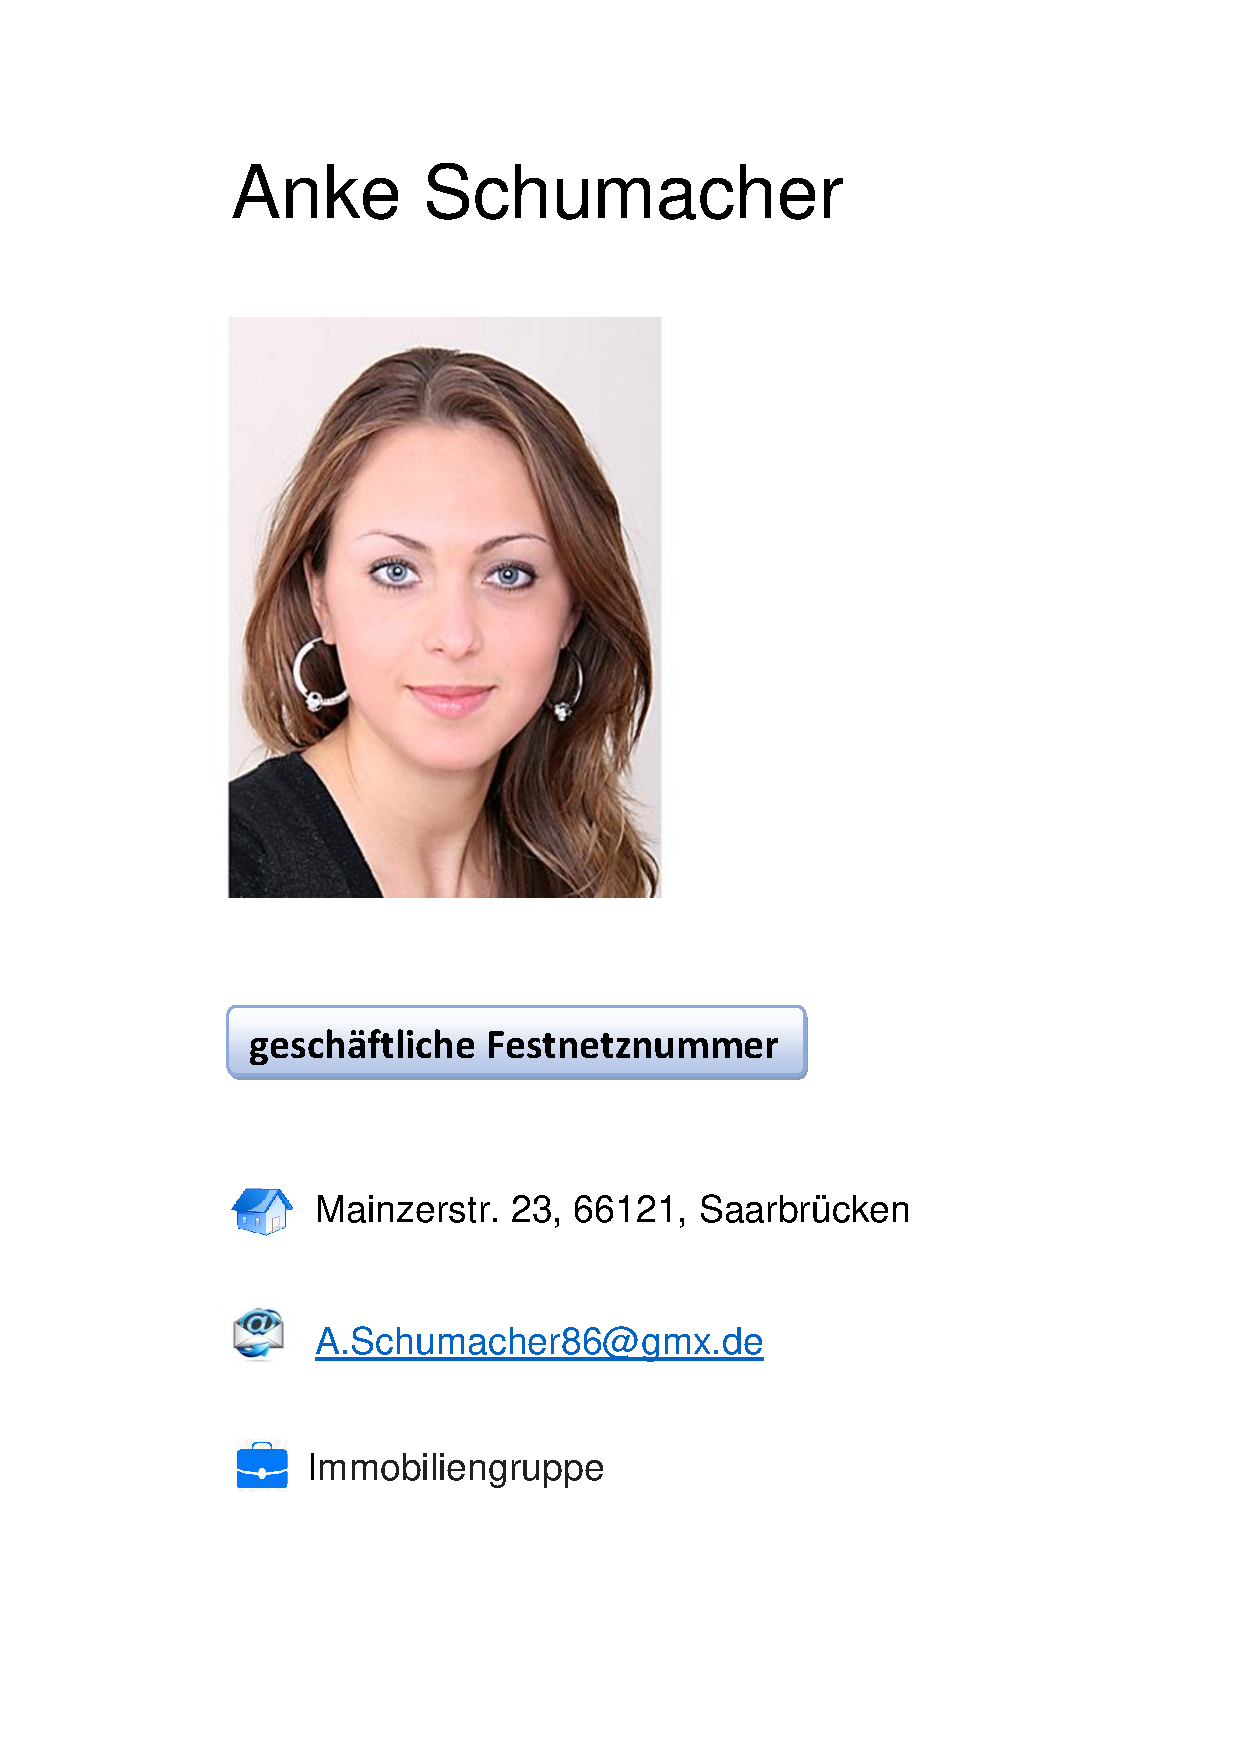
\includegraphics[width=12cm]{Anke2.pdf}
\caption{Personenprofil: Anke im 2. Versuch}
\label{anke2}
\end{center}
\end{figure}

Welche Slots pro Person abgefragt werden, zeigt Tabelle \ref{slotsPerson2}. 
Für jede Person werden zwei Slots abgefragt. Bei jedem der anzurufenden Kontakte wird nach dem Telefontyp gefragt, da für diesen Slot nur vier Füller möglich sind. Die Verteilung des zweiten Slots ist unterschiedlich.

\begin{longtable}{p{3,2cm}p{3,2cm}p{3,2cm}p{3,2cm}}
	\label{slotsPerson2}\\
	\caption[Slotabfrage pro Person]{Slotabfrage pro Person}\\
	\hline
	\textbf{Anke}&\textbf{Peter}&\textbf{Fritz} &\textbf{Kim}\\
	\hline
	\endfirsthead
	\hline
	\textbf{Anke}&\textbf{Peter}&\textbf{Fritz} &\textbf{Kim}\\
	\hline
	\endhead
Typ & Typ & Typ & Typ\\
Nachname & & & Nachname \\
& Firma & & \\
& & Stadt & \\

\hline
\end{longtable}


\subsection{Versuchsaufbau}
Der Versuchsaufbau ist identisch zu dem aus Versuch 1.
Tabelle \ref{ablauf} zeigt einen Überblick.

\begin{longtable}{p{2,4cm}p{2,4cm}p{2,4cm}p{2,4cm}p{2,4cm} }
	\label{ablauf}\\
	\caption[Übersicht Versuchsablauf]{Übersicht Versuchsablauf}\\
	\hline
	\textbf{Vorrunde}&\textbf{1. Runde}&\textbf{2. Runde} &\textbf{3. Runde} & \textbf{4. Runde}\\
	\hline
	\endfirsthead
	\hline
	\textbf{Vorrunde}&\textbf{1. Runde}&\textbf{2. Runde} &\textbf{3. Runde} \textbf{4. Runde}\\
	\hline
	\endhead
Rennspiel & Rennspiel & Rennspiel & Rennspiel &\\
 & Anruf Anke & Anruf Peter & Anruf Fritz & Anruf Kim \\
\hline
\end{longtable}

\subsection{Versuchsdesign}
Das Versuchsdesign wurde ebenfalls aus dem ersten Versuch übernommen.
Ein Überblick der Strecken- und Strategieverteilung pro Gruppe ist in Tabelle \ref{verteilung} aufgelistet. 

\begin{longtable}{p{3cm}p{3cm}p{3cm}p{3cm} }
	\label{verteilung}\\
	\caption[Strecken- und Strategieverteilung]{Strecken- und Strategieverteilung}\\
	\hline
	\textbf{Aufteilung}&\textbf{Strategie 1}&\textbf{Strategie 2} &\textbf{Strategie 3}\\
	\hline
	\endfirsthead
	\hline
	\textbf{Aufteilung}&\textbf{Strategie 1}&\textbf{Strategie 2} &\textbf{Strategie 3}\\
	\hline
	\endhead
1. Gruppe & Strecke A & Strecke B & Strecke C \\
2. Gruppe & Strecke B & Strecke C & Strecke A \\
3. Gruppe  & Strecke C & Strecke A & Strecke B \\
4. Gruppe   & keine Strecke & keine Strecke & keine Strecke\\ 
\hline
\end{longtable}

\subsection{Control Panel}
Das Control Panel aus Versuch 1 wurde mit anderen Sprachausgaben ausgestattet und es wurden weitere Schaltflächen für Strategie 3 hinzugefügt. (Abbildung \ref{cp2})
\begin{figure}[H]
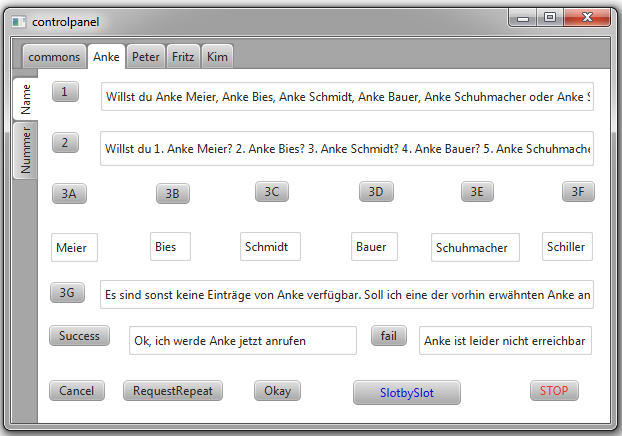
\includegraphics[width=13cm]{controlpanel2.png}
\caption{Controlpanel 2. Versuch}
\label{cp2}
\end{figure}


\subsection{Versuchspersonen}

Hier wurden ebenfalls 12 Muttersprachler getestet. Die Alterspanne der Probanden liegt zwischen 18 und 53. Jede Versuchsperson wurde zufällig einer Gruppe zugewiesen und hatte die selbe Aufgabe wie die Versuchsperson in Versuch 1: 
\begin{enumerate}
\item Testrunde fahren
\item Fragebogen über Person ausfüllen (siehe \ref{fbperson1} Unterkapitel Person)
\item Strecke A fahren + Anke anrufen
\item Fragebogen über kognitive Belastung und letzten Dialog ausfüllen (siehe \ref{fragebogen1} Unterkapitel Fragebogen)
\item Strecke B fahren + Peter anrufen
\item Fragebogen über kognitive Belastung und letzten Dialog ausfüllen
\item Strecke C fahren + Fritz anrufen
\item Fragebogen über kognitive Belastung und letzten Dialog ausfüllen 
\item Kim anrufen
\item Fragebogen über kognitive Belastung und letzten Dialog ausfüllen 
\end{enumerate}

Wie in Versuch 1 war die Aufgabe der Versuchspersonen ihre Eingaben deutlich über ein Tischmikrofon zu übermitteln. Dabei konnten sie sich die Personenprofile während des Dialoges auf einem Laptop ansehen.



\subsection{Auswertung}
\label{auswertung2}
Wie in Versuch 1 werden die Zeiten gemessen, die die Versuchsperson zum einen für das absolvieren der Strecke und zum anderen für das erfolgreiche Abschließen des Testszenarios benötigt (\ref{messwerte1} Gemessene Zeiten).
Nach jeder Rennrunde wird die Versuchsperson ebenfalls einen Fragebogen ausfüllen, welcher sich auf die subjektiv wahrgenommene kognitive Belastung und auf Merkmale der Disambiguierungsstrategien bezieht (\ref{fragebogen2} Fragebogen). Ebenfalls wird die Task Completion ausgewertet (\ref{TC2} Task Completion) und das Dialogverhalten untersucht (\ref{DV2} Dialogverhalten). Die erzielten Werte werden mit dem Tukey-Test
auf statistische Signifikanz geprüft. 
\subsubsection{Gemessene Zeiten}
\label{messwerte}
\paragraph{Rennzeiten} 
~\\
%\textbf{Rennzeiten}\\
In jeder Runde wurden die Rennzeiten bemessen. Mit diesen möchte man ermitteln, ob das Rennverhalten von einer Dialogstrategie beeinflusst wird. 
Die durchschnittlichen Rennzeiten für alle Strategien auf die einzelnen Strecken verteilt sind in Tabelle \ref{RZ3SV2} gelistet. 
\begin{longtable}{p{3cm}p{3cm}p{3cm}p{3cm} }
	\label{RZ3SV2}\\
	\caption[Durchschnittszeiten Strategie pro Strecke]{Durchschnittszeiten Strategie pro Strecke}\\
	\hline
	\textbf{Rennzeiten}&\textbf{Strategie 1}&\textbf{Strategie 2} &\textbf{Strategie 3}\\
	\hline
	\endfirsthead
	\hline
	\textbf{Rennzeiten}&\textbf{Strategie 1}&\textbf{Strategie 2} &\textbf{Strategie 3}\\
	\hline
	\endhead
Strecke A & 81 sek & 80,3 sek & 74,25 sek \\
Strecke B & 74,5 sek & 84,25 sek & 88 sek \\
Strecke C & 75 sek & 67,9 sek & 65 sek \\
\hline
\end{longtable}

Durch diese Ergebnisse kann man keine Strategie bestimmen, mit der die Strecken am besten bzw. am schlechtesten gefahren wurden.
Dies könnte daran liegen, dass einzelne Werte durch schlechtere bzw. bessere Spieler in den Gruppen verfälscht wurden. Tabelle \ref{RennZeitenDis2} beinhaltet die durchschnittlichen Rennzeiten aller Strecken pro Strategie. 

\begin{longtable}{p{3cm}p{3cm}p{3cm}p{3cm} }
	\label{RennZeitenDis2}\\
	\caption[Durchschnittszeiten pro Strategie]{Durchschnittszeiten pro Strategie}\\
	\hline
	\textbf{Rennzeiten}&\textbf{Strategie 1}&\textbf{Strategie 2} &\textbf{Strategie 3}\\
	\hline
	\endfirsthead
	\hline
	\textbf{Rennzeiten}&\textbf{Strategie 1}&\textbf{Strategie 2} &\textbf{Strategie 3}\\
	\hline
	\endhead
Durschnitt & 76,83 sek & 77,47 sek & 76,73 sek \\
\hline
\end{longtable}
Die Zeiten weichen nur sehr gering voneinander ab und die Unterschiede sind zudem statistisch nicht signifikant. Diese Erkenntnis bekräftigt die in Versuch 1 getroffene Vermutung, dass die Rennzeit keinen Aufschluss darüber gibt, welche Strategie für die Autofahrt am Geeignetsten ist. 

\paragraph{Dialogzeiten}
~\\
Neben den Zeiten für das Rennspiel werden auch die Dialogzeiten berechnet. 
Die Werte daraus werden dazu genutzt, um zu erforschen, mit welcher Strategie der kürzeste Dialog möglich ist. Weiter werden aufkommende Unterschiede im Dialogverhalten zwischen einer hoch belastenden und eine weniger belasteten Versuchsperson untersucht. 
Es werden alle Dialogzeiten aus den Runden mit Rennspiel gemessen und einmal für jede Strecke der Durchschnitt pro Strategie und einmal der gesamte Durchschnitt pro Strategie gebildet. Diese Werte lassen sich gegen die Durchschnittszeiten aus der Runde ohne Rennspiel vergleichen. Es werden allerdings nur die Zeiten gewertet, bei denen der Dialog eine maximale Task Completion erreicht hat.
In Tabelle \ref{Durchschnittsdialogzeiten2} sind die Durchschnittszeiten der gemessenen Runden aufgelistet.

\begin{longtable}{p{3cm}p{3cm}p{3cm}p{3cm} }
	\label{Durchschnittsdialogzeiten2}\\
	\caption[Durchschnittsdialogzeiten 2. Versuch]{Durchschnittsdialogzeiten 2. Versuch}\\
	\hline
	\textbf{Dialogzeiten}&\textbf{Strategie 1}&\textbf{Strategie 2} &\textbf{Strategie 3}\\
	\hline
	\endfirsthead
	\hline
	\textbf{Rennzeiten}&\textbf{Strategie 1}&\textbf{Strategie 2} &\textbf{Strategie 3}\\
	\hline
	\endhead
Strecke A & 25,76 sek & 38,32 sek & 33,98 sek \\
Strecke B & 31,41 sek & 40,2 sek & 36,61 sek \\
Strecke C  & 29,59 sek & 37,9 sek & 28,29 sek \\
\hline
\hline
Strecke A - C & 29,55 sek & 38,54 sek & 34,34 sek\\
\hline
ohne Strecke & 24,12 & 34,35 & 30,44 \\
\hline
\end{longtable}

Die zeitlichen Unterschiede der Disambiguierungsstrategien sind statistisch signifikant. An diesem Ergebnis sieht man, dass die erste Strategie den kürzesten Dialog ermöglicht und die zweite Strategie im Durchschnitt am Längsten dauert. Dies gilt sowohl für die Runden mit als auch für die Runden ohne Rennspiel. Der Vergleich der letzten beiden Zeilen der Tabelle macht deutlich, dass auch in diesem Versuch der Dialog ohne Rennspiel im Durchschnitt deutlich kürzer war, als der Dialog mit Rennspiel. Dadurch wird vermutet, dass die Reaktionszeit bei geringer Belastung kleiner ist, als bei höherer Belastung.  

\subsubsection{Fragebogen}
\label{fragebogen2}
Zu Beginn des Versuchs wird derselbe Personenfragenbogen wie in Versuch 1 ausgefüllt. Nach jeder Runde wird ebenfalls der Fragebogen, bestehend aus einem Teil des NASA-TLX Tests und einem Teil über die zuletzt gehörten Strategie, abgefragt.

\paragraph{Nasa-TLX}
~\\
Dieser Teil des Fragebogens wird wie im ersten Versuch dazu genutzt um zu erforschen, bei welcher Strategie eine höhere Belastung empfunden wurde und ob es Unterschiede in der empfundenen Belastung in den Runden mit und ohne Rennspiel gibt. 
Die nachfolgende Tabelle zeigt die Ergebnisse jeder Frage pro Strategie.
\newpage
\begin{longtable}{|p{4cm}|p{2cm}|p{2cm}|p{2cm}|p{2cm}|}
	\hline
		\textbf{Antwortenintervall}&\textbf{Strategien}&\multicolumn{3}{c|}{\textbf{Ergebnisse bestimmter Runden}}\\
	&&\textbf{1-4}&\textbf{1-3} &\textbf{4}\\
	\hline
	\endfirsthead
	\hline
	\textbf{Antwortenintervall}&\textbf{Strategien}&\textbf{Runden 1-4}&\textbf{Runden 1-3} &\textbf{Runde 4}\\
	\hline
	\endhead
		\multicolumn{5}{l}{\textbf{Geistige Anforderung}}\\
		\hline
\multirow{3}{4cm}{1: gering \newline 6: hoch} & Strategie 1 &  2,31 & 2,67 & 1,25 \\
 & Strategie 2 & 2,31 & 2,58 & 1,5\\
 & Strategie 3 & 2,56 & 2,83 & 1,75 \\
\hline
		\multicolumn{5}{l}{\textbf{Körperliche Anforderung}}\\
		\hline
\multirow{3}{4cm}{1: gering \newline 6: hoch} & Strategie 1 & 1,67 & 2,17 & 1 \\
 & Strategie 2 & 2,06 & 2,25 & 1,5 \\
 & Strategie 3 & 1,94 & 2,08 & 1,5 \\
\hline
		\multicolumn{5}{l}{\textbf{Zeitliche Anforderung}}\\
		\hline
\multirow{3}{4cm}{1: gering \newline 6: hoch} & Strategie 1 & 2 & 2,25 & 1,25 \\
 & Strategie 2 & 2,25 & 2,5 & 1,5 \\
 & Strategie 3 & 1,94 & 2,17 & 1,25 \\
\hline
		\multicolumn{5}{l}{\textbf{Leistung}}\\
		\hline
\multirow{3}{4cm}{1: gering \newline 6: hoch} & Strategie 1 & 5,13 & 4,83 & 6 \\
 & Strategie 2 & 4,88 & 4,67 & 5,5 \\
 & Strategie 3 & 4,56 & 4,08 & 6 \\
\hline
		\multicolumn{5}{l}{\textbf{Anstrengung}}\\
		\hline
\multirow{3}{4cm}{1: gering \newline 6: hoch} & Strategie 1 & 2,38 & 2,83 & 1 \\
 & Strategie 2 & 2,44 & 2,67 & 1,75 \\
 & Strategie 3 & 2,31 & 2,67 & 1,25\\
\hline
		\multicolumn{5}{l}{\textbf{Frustration}}\\
		\hline
\multirow{3}{4cm}{1: gering \newline 6: hoch} & Strategie 1 & 1,94 & 2,25 & 1 \\
 & Strategie 2 & 1,94 & 2 & 1,75 \\
 & Strategie 3 & 2,31 & 2,58 & 1,5 \\
\hline
\end{longtable}

Auch in diesem Versuch sind die Antworten der einzelnen Strategien rein statistisch nicht signifikant unterschiedlich und es ist kein eindeutiges Muster zu erkennen, welche Strategie am Wenigsten belastend ist. 
Beim Vergleich der Antworten von Runde 1-3 mit Runde 4 wird jedoch deutlich, dass bei allen Fragen die Runde mit Rennspiel als belastender gewertet wurde als die Runde ohne. Dieses Ergebnis bestätigt das Ergebnis aus Versuch 1 und bestärkt die Aussage, dass hier ein Unterschied in der Belastung empfunden worden ist.  

\paragraph{Strategien}
~\\
In diesem Fragebogen bewerten die Versuchspersonen die zuletzt verwendete Strategie anhand verschiedener Kategorien. Die Durchschnittsantworten sind in nachfolgenden Tabelle aufgelistet. 
\newpage
\begin{longtable}{|p{4cm}|p{2cm}|p{2cm}|p{2cm}|p{2cm}|}
	\hline
		\textbf{Antwortenintervall}&\textbf{Strategien}&\multicolumn{3}{c|}{\textbf{Ergebnisse bestimmter Runden}}\\
	&&\textbf{1-4}&\textbf{1-3} &\textbf{4}\\
	\hline
	\endfirsthead
	\hline
	\textbf{Antwortenintervall}&\textbf{Strategien}&\textbf{Runden 1-4}&\textbf{Runden 1-3} &\textbf{Runde 4}\\
	\hline
	\endhead
		\multicolumn{5}{l}{\textbf{Der Dialog lenkte mich vom Rennspiel ab}}\\
		\hline
\multirow{3}{4cm}{1: kaum \newline 6: stark} & Strategie 1 & - & 3,5  & - \\
 - & Strategie 2 & - & 2,92 & -\\
 - & Strategie 3 & - & 3,17 & -\\
\hline
		\multicolumn{5}{l}{\textbf{Die Nachfragen erleichterten es mir, den Anruf korrekt aufzubauen}}\\
		\hline
\multirow{3}{4cm}{1: erleichterte es\newline  6: erschwerte es} & Strategie 1 & 2,44 & 2,58 & 2 \\
 & Strategie 2 & 2,25 & 2,33 & 2 \\
 & Strategie 3 & 2,38 & 2,5 & 2 \\
\hline
		\multicolumn{5}{l}{\textbf{Wussten Sie, wann das System Spracheingaben erwartete?}}\\
		\hline
\multirow{3}{4cm}{1: immer \newline  6: nicht immer} & Strategie 1 & 1,63 & 1,67 & 1,5 \\
 & Strategie 2 & 1,5 & 1,5 & 1,5 \\
 & Strategie 3 & 1,57 & 1,5 & 1,75 \\
\hline
		\multicolumn{5}{l}{\textbf{Wie gefiel Ihnen der Dialog insgesamt?}}\\
		\hline
\multirow{3}{4cm}{1: sehr gut \newline  6: weniger gut} & Strategie 1 & 2,94 & 2,83 & 3,25 \\
 & Strategie 2 & 2,44 & 2,42 & 2,5 \\
 & Strategie 3 & 2,38 & 2,3 & 2,5 \\
\hline
		\multicolumn{5}{l}{\textbf{Fiel es Ihnen einfacher, den Dialog ohne Rennspiel zu führen?}}\\
		\hline
\multirow{3}{4cm}{1: viel einfacher \newline  6: nicht einfacher} & Strategie 1 & - & - & 2,75 \\
- & Strategie 2 & - & - & 3 \\
- & Strategie 3 & - & - & 2,5\\
\hline
		\multicolumn{5}{l}{\textbf{Welcher Anruf gefiel Ihnen insgesamt am besten?}}\\
		\hline
\multirow{3}{4cm}{Anruf bzw. Strategie auswählbar} & Strategie 1 & 16,7\% &-  &-  \\
 & Strategie 2 & 33,3\% & - & - \\
 & Strategie 3 & 50\% & - &  -\\
\hline
\end{longtable}

Es kann keine Strategie identifiziert werden, die eindeutig am besten bewertet wurde. 
Die Fragen im Bezug auf Ablenkung, erleichtertet Aufbau durch Nachfragen und Zeitpunkt der Spracheingaben wurden für Strategie 2 am besten bewertet.
Die Frage \texttt{"Wie gefiel Ihnen der Dialog insgesamt"} erhielt für Strategie 3 den höchsten Wert. Dadurch gefiel den Versuchspersonen diese Dialogstrategie am besten. Diese Erkenntnis wird durch das Ergebnis der letzten Frage bestätigt, welche konkret nach der besten Strategie fragt. Auf diese Frage wurde am häufigsten mit Strategie 3 geantwortet. Parallel gilt dies für Strategie 1, welche den niedrigster Wert erhielt und auch am seltensten bei der letzten Frage gewählt wurde. \\

Die vorletzte Frage zeigt, dass es leichter fiel, den Dialog ohne Rennspiel zu führen und bestätigt damit auch hier das Ergebnis des NASA-TLX-Tests.

\paragraph{Person}
\label{fbperson1}
~\\
In diesem Versuch werden die gleichen Informationen über die Versuchsperson zu Beginn des Fragebogens abgefragt. (vgl Abbildung \ref{fbperson})\\

42\% der Probanten sind in einer Altersgruppe von 18-29, 25 \% in einer Altersgruppe von 30-41 und 33\% in einer Altersgruppe von 42-53. Alle Versuchspersonen sind deutsche Muttersprachler. 
Eine Zusammenfassung der restlichen Antworten steht in Abbildung \ref{fbpersonaus2}.


\begin{figure}[H]
\begin{center}
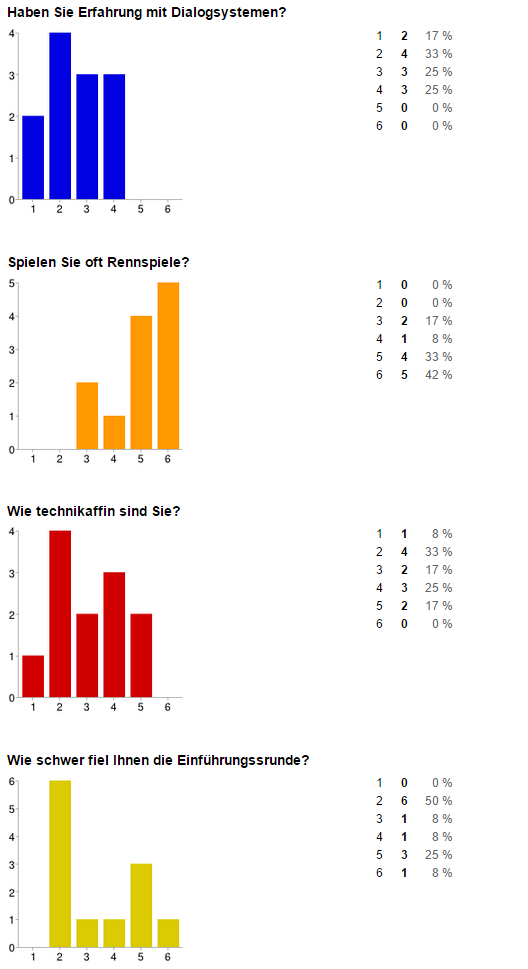
\includegraphics[width=10cm]{person2.png}
\caption{Fragebogen: Person}
\label{fbpersonaus2}
\end{center}
\end{figure}
\newpage

Das Ergebnis zeigt, dass 75\% der Testpersonen keine bzw. wenig Erfahrung mit Dialogsystemen haben. Aus den Antworten lässt sich weiter schließen, dass 83\% der Befragten selten Rennspiele spielen und die Einführungsrunde 58\% schwer fiel. Diese Prozentangaben stimmen zufällig mit den Zahlen aus dem ersten Versuch überein. Dadurch kann ausgeschlossen werden, dass die Unterschiede der Resultate aus beiden Versuchen durch unterschiedliche Erfahrung der Versuchspersonen mit Dialogsystemen und Rennspielen zustande kommen. 


\subsubsection{Task Completion}
\label{TC2}
Für jede Strategie wird ebenfalls die Task Completion ausgewertet, welche besagt, mit welchem Erfolg der Anruf ausgeführt wurde. Folgende Punktezahlen sind für jede Strategie möglich:
\begin{itemize}
\item 0 Punkte, wenn kein Slot richtig gefüllt wird
\item 1 Punkt, wenn ein Slot richtig gefüllt wird
\item 2 Punkte, wenn alle Slots richtig gefüllt werden
\end{itemize}
Zur Auswertung wird pro Strategie eine Durchschnittspunktzahl berechnet, welche in Tabelle \ref{TCV2} stehen. 

\begin{longtable}{p{3cm}p{3cm}p{3cm}p{3cm} }
	\label{TCV2}\\
	\caption[Task Completion Versuch 2]{Task Completion Versuch 2}\\
	\hline
\textbf{Strategien}&\textbf{insgesamt}&\textbf{Runde 1-3} &\textbf{Runde 4}\\
	\hline
	\endfirsthead
	\hline
	\textbf{Strategien}&\textbf{\O TC insgesamt}&\textbf{\O TC Runde 1-3} &\textbf{\O TC Runde 4}\\
	\hline
	\endhead
1. Strategie & 1,88 & 1,83 & 2  \\
2. Strategie & 1,81 & 1,75 & 2  \\
3. Strategie & 1,56 & 1,42 & 2  \\
\hline
Insgesamt & & 1,67 & 2 \\ 
\hline
\end{longtable}

Hier zeigt sich klar, dass die Dialoge in Runde 4 ohne Fehler erfolgten und somit im Durchschnitt erfolgreicher waren als die Runden mit Rennspiel. Es fällt auf, dass die Strategie, die in diesem Versuch als am Beliebtesten ausgewertet wurde, am meisten Fehler aufweist. Dabei kommt erneut die Frage aus Versuch 1 auf, ob man hier eine Verbindung zwischen beliebtester Strategie und Task Completion ziehen kann und ob die Versuchspersonen bemerkten, dass sie die Slots falsch gefüllt haben. 
Grundsätzlich kann man an diesem Ergebnis sehen, dass insgesamt ein Anruf am häufigsten korrekt mit Strategie 1 und am seltensten korrekt mit Strategie 3 ausgeführt werden konnte. 

\subsubsection{Dialogverhalten}
\label{DV2}
In diesem Versuch wurde mit denselben Antwortmöglichkeiten geantwortet wie in Versuch 1 (siehe Tabelle \ref{Dialogverhalten11}).

Die Häufigkeiten dieser Antworten pro Strategie aus Runde 1-3 sind in nachfolgender Tabelle aufgelistet.

\begin{longtable}{p{3cm}p{3cm}p{3cm}p{3cm} }
	\label{Dialogverhalten12}\\
	\caption[Antwortenverteilung pro Strategie]{Antwortenverteilung pro Strategie}\\
	\hline
\textbf{Antwort-möglichkeiten}&\textbf{Strategie 1}&\textbf{Strategie 2} &\textbf{Strategie 3}\\
	\hline
	\endfirsthead
	\hline
	\textbf{Antwortmöglichkeiten}&\textbf{Strategie 1}&\textbf{Strategie 2} &\textbf{Strategie 3}\\
	\hline
	\endhead
Slots & 100\% & 62,5\%\ & 0\%  \\
Position & 0\% & 37,5\% & 0\%  \\
ja/nein & 0\% & 0\%  & 100 \%  \\
\hline
\end{longtable}
Diese Ergebnisse sind mit denen aus Versuch 1 zu vergleichen. 
Hier wurde bei hoher Belastung ebenfalls mit den gleichen Antwortmöglichkeiten geantwortet wie bei niedriger Belastung, weshalb kein Unterschied im Dialogverhalten bei unterschiedlicher Belastung erkennbar ist. 




\subsection{Resultat}
Aus den Resultaten aus Kapitel \ref{auswertung2} wird die effizienteste Strategie ermittelt. \newline

Durch die Dialogzeiten wird klar, dass Strategie 1 sowohl in den Runden mit, sowie ohne Rennspiel den kürzesten Dialog ermöglicht. Aus den Ergebnissen des NASA-TLX Fragebogens und den Rennzeiten kann kein Rückschluss auf die effizienteste Strategie gezogen werden. Der zweite Teil des Fragebogens zeigt, dass Strategie 2 weniger ablenkt, einfacher aufzubauen ist und man den Zeitpunkt der Spracheingaben einfacher erkennt. Strategie 3 gefiel den Versuchspersonen allerdings am besten. Die Task Completion zeigt jedoch, dass Strategie 3 insgesamt am Schlechtesten und Strategie 1 am besten abschnitt. \newline
Durch dieses Ergebnis wird Strategie 1 aufgrund der kürzesten Dialogzeit und der besten Task Completion als effizienteste Strategie gewertet. Strategie 3 ist jedoch eindeutig die Beliebteste. 

\begin{comment}
\subsubsection{Zeiten}
\paragraph{Rennzeiten}
~\\
\begin{longtable}{p{3cm}p{3cm}p{3cm}p{3cm} }
	\label{durchschnittsvorl}\\
	\caption[Durchschnittszeiten Strategie pro Strecke]{Durchschnittszeiten Strategie pro Strecke}\\
	\hline
	\textbf{Rennzeiten}&\textbf{Strategie 1}&\textbf{Strategie 2} &\textbf{Strategie 3}\\
	\hline
	\endfirsthead
	\hline
	\textbf{Rennzeiten}&\textbf{Strategie 1}&\textbf{Strategie 2} &\textbf{Strategie 3}\\
	\hline
	\endhead
Strecke A & 81 sek & 80,3 sek & 74,25 sek \\
Strecke B & 74,5 sek & 84,25 sek & 88 sek \\
Strecke C & 75 sek & 67,9 sek & 65 sek \\
\hline
Strecke A - C & 76,83 & 77,47 & 76,73 \\
\hline
\end{longtable}

\paragraph{Dialogzeiten}
~\\

\begin{longtable}{p{3cm}p{3cm}p{3cm}p{3cm} }
	\label{durchschnittsvorl}\\
	\caption[Durchschnittszeiten Strategie pro Strecke]{Durschnittszeiten Strategie pro Strecke}\\
	\hline
	\textbf{Dialogzeiten}&\textbf{Strategie 1}&\textbf{Strategie 2} &\textbf{Strategie 3}\\
	\hline
	\endfirsthead
	\hline
	\textbf{Rennzeiten}&\textbf{Strategie 1}&\textbf{Strategie 2} &\textbf{Strategie 3}\\
	\hline
	\endhead
Strecke A & 25,76 sek & 38,32 sek & 33,98 sek \\
Strecke B & 31,41 sek & 40,2 sek & 36,61 sek \\
Strecke C  & 29,59 sek & 37,9 sek & 28,29 sek \\
\hline
\hline
Strecke A - C & 29,55 sek & 38,54 sek & 34,34 sek\\
\hline
ohne Strecke & 24,12 & 34,35 & 30,44 \\
\hline
\end{longtable}
 
\begin{longtable}{p{4cm}p{4cm}p{4cm}}
	\label{Dialogzeiten13vs4}\\
	\caption[Durschnittszeiten mit Rennspiel versus ohne Rennspiel]{Durschnittszeiten mit Rennspiel versus ohne Rennspiel}\\
	\hline
	\textbf{Dialogzeiten}&\textbf{Runde 1-3}&\textbf{Runde 4}\\
	\hline
	\endfirsthead
	\hline
	\textbf{Dialogzeiten}&\textbf{Runde 1-3}&\textbf{Runde 4}\\
	\hline
	\endhead
Durschnitt &  34,64 sek & 29,63 sek \\


\hline
\end{longtable}

\subsubsection{Fragebogen}
\paragraph{Nasa-TLX}
~\\
\begin{longtable}{|p{4cm}|p{2cm}|p{2cm}|p{2cm}|p{2cm}|}
	\hline
		\textbf{Antwortenintervall}&\textbf{Strategien}&\multicolumn{3}{c|}{\textbf{Ergebnisse bestimmter Runden}}\\
	&&\textbf{1-4}&\textbf{1-3} &\textbf{4}\\
	\hline
	\endfirsthead
	\hline
	\textbf{Antwortenintervall}&\textbf{Strategien}&\textbf{Runden 1-4}&\textbf{Runden 1-3} &\textbf{Runde 4}\\
	\hline
	\endhead
		\multicolumn{5}{l}{\textbf{Geistige Anforderung}}\\
		\hline
\multirow{3}{4cm}{1: gering \newline 6: hoch} & Strategie 1 &  2,31 & 2,67 & 1,25 \\
 & Strategie 2 & 2,31 & 2,58 & 1,5\\
 & Strategie 3 & 2,56 & 2,83 & 1,75 \\
\hline
		\multicolumn{5}{l}{\textbf{Körperliche Anforderung}}\\
		\hline
\multirow{3}{4cm}{1: gering \newline 6: hoch} & Strategie 1 & 1,67 & 2,17 & 1 \\
 & Strategie 2 & 2,06 & 2,25 & 1,5 \\
 & Strategie 3 & 1,94 & 2,08 & 1,5 \\
\hline
		\multicolumn{5}{l}{\textbf{Zeitliche Anforderung}}\\
		\hline
\multirow{3}{4cm}{1: gering \newline 6: hoch} & Strategie 1 & 2 & 2,25 & 1,25 \\
 & Strategie 2 & 2,25 & 2,5 & 1,5 \\
 & Strategie 3 & 1,94 & 2,17 & 1,25 \\
\hline
		\multicolumn{5}{l}{\textbf{Leistung}}\\
		\hline
\multirow{3}{4cm}{1: gering \newline 6: hoch} & Strategie 1 & 5,13 & 4,83 & 6 \\
 & Strategie 2 & 4,88 & 4,67 & 5,5 \\
 & Strategie 3 & 4,56 & 4,08 & 6 \\
\hline
		\multicolumn{5}{l}{\textbf{Anstrengung}}\\
		\hline
\multirow{3}{4cm}{1: gering \newline 6: hoch} & Strategie 1 & 2,38 & 2,83 & 1 \\
 & Strategie 2 & 2,44 & 2,67 & 1,75 \\
 & Strategie 3 & 2,31 & 2,67 & 1,25\\
\hline
		\multicolumn{5}{l}{\textbf{Frustration}}\\
		\hline
\multirow{3}{4cm}{1: gering \newline 6: hoch} & Strategie 1 & 1,94 & 2,25 & 1 \\
 & Strategie 2 & 1,94 & 2 & 1,75 \\
 & Strategie 3 & 2,31 & 2,58 & 1,5 \\
\hline
\end{longtable}


\paragraph{Strategien}
~\\
\begin{longtable}{|p{4cm}|p{2cm}|p{2cm}|p{2cm}|p{2cm}|}
	\hline
		\textbf{Antwortenintervall}&\textbf{Strategien}&\multicolumn{3}{c|}{\textbf{Ergebnisse bestimmter Runden}}\\
	&&\textbf{1-4}&\textbf{1-3} &\textbf{4}\\
	\hline
	\endfirsthead
	\hline
	\textbf{Antwortenintervall}&\textbf{Strategien}&\textbf{Runden 1-4}&\textbf{Runden 1-3} &\textbf{Runde 4}\\
	\hline
	\endhead
		\multicolumn{5}{l}{\textbf{Der Dialog lenkte mich vom Rennspiel ab}}\\
		\hline
\multirow{3}{4cm}{1: kaum \newline 6: stark} & Strategie 1 & \multirow{3}{2,5cm}{in Runde 4 nicht beantwortet} & 3,5  & \multirow{3}{2,5cm}{nicht beantwortet} \\
 & Strategie 2 & & 2,92 & \\
 & Strategie 3 & & 3,17 & \\
\hline
		\multicolumn{5}{l}{\textbf{Die Nachfragen erleichterten es mir, den Anruf korrekt aufzubauen}}\\
		\hline
\multirow{3}{4cm}{1: erleichterte es\newline  6: erschwerte es} & Strategie 1 & 2,44 & 2,58 & 2 \\
 & Strategie 2 & 2,25 & 2,33 & 2 \\
 & Strategie 3 & 2,38 & 2,5 & 2 \\
\hline
		\multicolumn{5}{l}{\textbf{Wussten Sie, wann das System Spracheingaben erwartete?}}\\
		\hline
\multirow{3}{4cm}{1: immer \newline  6: nicht immer} & Strategie 1 & 1,63 & 1,67 & 1,5 \\
 & Strategie 2 & 1,5 & 1,5 & 1,5 \\
 & Strategie 3 & 1,57 & 1,5 & 1,75 \\
\hline
		\multicolumn{5}{l}{\textbf{Wie gefiel Ihnen der Dialog insgesamt?}}\\
		\hline
\multirow{3}{4cm}{1: sehr gut \newline  6: weniger gut} & Strategie 1 & 2,94 & 2,83 & 3,25 \\
 & Strategie 2 & 2,44 & 2,42 & 2,5 \\
 & Strategie 3 & 2,38 & 2,3 & 2,5 \\
\hline
		\multicolumn{5}{l}{\textbf{Fiel es Ihnen einfacher, den Dialog ohne Rennspiel zu führen?}}\\
		\hline
\multirow{3}{4cm}{1: viel einfacher \newline  6: nicht einfacher} & Strategie 1 & \multirow{3}{2,5cm}{in Runden 1-3 nicht beantwortet} & \multirow{3}{2,5cm}{nicht beantwortet} & 2,75 \\
 & Strategie 2 & & & 3 \\
 & Strategie 3 & & & 2,5\\
\hline
		\multicolumn{5}{l}{\textbf{Welcher Anruf gefiel Ihnen insgesamt am besten?}}\\
		\hline
\multirow{3}{4cm}{Anruf bzw. Strategie auswählbar} & Strategie 1 & 16,7\% & & \\
 & Strategie 2 & 33,3\% && \\
 & Strategie 3 & 50\% && \\
\hline
\end{longtable}
\subsubsection{Task Completion}
\begin{longtable}{p{3cm}p{3cm}p{3cm}p{3cm} }
	\label{Dialogzeiten}\\
	\caption[Durschnittliche Task Completion (TC)]{Durschnittliche Task Completion (TC)}\\
	\hline
\textbf{Strategien}&\textbf{insgesamt}&\textbf{Runde 1-3} &\textbf{Runde 4}\\
	\hline
	\endfirsthead
	\hline
	\textbf{Strategien}&\textbf{\O TC insgesamt}&\textbf{\O TC Runde 1-3} &\textbf{\O TC Runde 4}\\
	\hline
	\endhead
1. Strategie & 1,88 & 1,83 & 2  \\
2. Strategie & 1,81 & 1,75 & 2  \\
3. Strategie & 1,56 & 1,42 & 2  \\
\hline
Insgesamt & & 1,67 & 2 \\ 
\hline
\end{longtable}
Fragebogen: NASA-TLX\\
Wurde der Task zu ende geführt?\\
Wurde dem User klar, welche Eingaben er machen konnte (das erste, der zweite..)\\
Wurde richtig geantwortet?\\
Konkrete Zahlen besser als Benutzermeinung \\
wie einig sind sich die Benutzer\\
Extreme vorhanden?\\
wie kann man auswerten?
\begin{itemize}
\item Reaktionszeit
\item Taskdauer
\item Reaktion während Vorlesens bewerten
\item vergleich zeit mit und ohne CL
\item Interaktion bewerten lassen (skala 1-10)
 \begin{itemize}
\item Wie intuitiv 
\item angnehm?
\item ablenkend oder störend während der Fahrt?
\item wie aufmerksam musste man sein 

\end{itemize}
\end{itemize}

\end{comment}

\newpage
\section{Ergebnisse}
\label{Ergebnisse}

Durch die Ergebnisse der Versuche können die Strategien bezüglich verschiedener Komponenten auf Effizienz und Beliebtheit für eine automobile Anwendung getestet werden. \\
\\
Die Rennzeiten werden gemessen um zu überprüfen, ob eine Dialogstrategie das Rennverhalten stört. In keinem Versuch kann jedoch eine Strategie bestimmt werden, mit der die Rennstrecken am besten bzw. am schlechtesten gefahren werden. Die Unterschiede in den Zeiten der einzelnen Strategien sind zum Einen sehr gering und zum anderen statistisch nicht signifikant. Daher kann hier keine aussagekräftige Erkenntnis über eine effizienteste Strecke gezogen werden, da die Zeiten durch Zufall zustande gekommen sein könnten.\\
\\
Neben den Rennzeiten wurde die Dialogzeit gemessen. Dies soll eine Erkenntnis darüber geben, mit welcher Strategie der kürzeste Dialog möglich ist. Weiter kann erforscht werden, ob Unterschiede in der Reaktionszeit zwischen einer kognitiv hoch belasteten und einer weniger belasteten Versuchsperson zu erkennen sind. In beiden Versuchen ist in allen Runden der kürzeste Dialog mit Strategie 1 möglich. Durch einen Vergleich der Dialogzeiten der Runden mit und ohne Rennspiel wird deutlich, dass die Dialogzeiten in den Runden ohne Rennspiel besser sind. Da zwischen den Runden mit und ohne Rennspiel kein unterschiedliches Dialogverhalten zu erkennen ist, kann man die Unterschiede nicht darauf zurückführen. Dadurch wird stark vermutet, dass die Probanden bei geringerer kognitiver Belastung eine schnellere Reaktionszeit aufweisen als bei hoher Belastung. \\
\\
Durch den NASA-TLX Fragebogen nach jeder Runde wird analysiert, welche Strategie als am belastendsten empfunden wurde. Weiter soll aus den Antworten ermittelt werden, ob eine unterschiedliche Belastung zwischen den Runden mit und ohne Rennspiel gespürt wurde.  
Die Ergebnisse beider Versuche zeigen, dass keine Strecke eindeutig als am belastendsten gewertet wurde, zudem sind die Ergebnisse statistisch nicht signifikant. 
Der Vergleich der Antworten zwischen den Runden mit und ohne Rennspiel bestätigt die Aussage, dass die Probanden in den Runden mit Rennspiel in jedem Versuch eine höhere Belastung empfunden haben als in den Runden ohne. \\
\\
Der Fragebogen über die getesteten Strategien zeigt wie die Versuchsperson die Strategien in Bezug auf verschiedene Kategorien bewerten. Im ersten Versuch, indem nur über zwei mögliche Slotfüller disambiguiert wurde, ist Strategie 1 am besten bewertet worden. Strategie 1 wurde in diesem Fragebogen auch als beliebteste Strategie gewertet. Am schlechtesten wurde Strategie 3 bewertet. Diese Ergebnisse sind nicht deckungsgleich mit den Ergebnissen aus Versuch 2. Bei diesem wurde zwar keine Strategie eindeutig am besten bewertet, jedoch wurde Strategie 3 als beliebteste Strategie und Strategie 1 als unbeliebteste Strategie gewertet. Hier ist ein deutlicher Unterschied zwischen beiden Versuchen zu erkennen. Prinzipiell zeigt das Ergebnis, dass die Beliebtheit der Strategien von der Länge der Disambiguierung abhängt. Das Resultat lässt vermuten, dass bei kurzer Disambiguierung eine möglichst schneller Dialog bevorzugt wird. Bei längerer Disambiguierung wird die Strategie bevorzugt, bei der man das Tempo durch das Annehmen bzw. Ablehnen des vorgeschlagenen Slotfüllers selbst bestimmen kann. Dies wird bei einer langen Sprachausgabe wahrscheinlich dadurch bevorzugt, da man nicht ununterbrochen konzentriert dem Dialog folgen muss. Dies fällt bei einem kurzen Dialog einfacher. \\
\newline
Um zu analysieren, welche Strategie am erfolgreichsten ist, wurde die Task Completion für beide Versuche ausgewertet. Die Ergebnisse beider Versuche fallen unterschiedlich aus. Im ersten Versuch erzielte Strategie 2 die höchste Task Completion und im zweiten Versuch Strategie 1. In beiden Versuchen war Strategie 3 am wenigsten erfolgreich. Dies deckt sich jedoch nicht mit dem Ergebnis, dass diese Strategie in Versuch 2 als beliebteste gewertet wurde. In einer zukünftigen Arbeit könnte die Frage geklärt werden, ob man hier einen Zusammenhang zwischen beliebtester und erfolgreichster Strategie ziehen bilden kann. 
Durch die Task Completion beider Versuche kommt man jedoch zu dem Resultat, dass die Dialoge mit niedriger Belastung erfolgreicher durchgeführt wurden. \\
\newline
Für beide Versuche wurde zusätzlich überprüft, mit welchen Antworten auf Rückfragen reagiert wurde. Dabei ist auffällig, dass die Verteilung der Antworten auf die einzelnen Strategien bei beiden Versuchen sehr ähnlich ist. In beiden Versuchen konnte zudem kein Unterschied im Dialogverhalten bei unterschiedlicher Belastung erkannt werden. \\
\newline
Zusammenfassend zeigen die Ergebnisse der beiden Versuche insgesamt, dass die Disambiguierungslänge bei der Bewertung der Strategien eine Rolle spielt. Bei der Formulierung einer Disambiguierung im Dialogsystem für das Auto, sollte der Dialogdesigner die Anzahl der möglichen Slotfüller beachten. Der erste Versuch zeigt deutlich, dass bei einer Disambiguierung über wenige Slotfüller eine Rückfrage in Strategie 1 am geeignetsten ist. Je nachdem ob auf Beliebtheit unter den Benutzern oder auf Effizienz  wert gelegt wird, sollte sich bei längere Disambiguierung für Strategie 1 oder Strategie 3 entschieden werden. 


\section{Diskussion}
\label{discussion}
In dieser Arbeit wurden zwei Versuche durchgeführt um drei Strategien auf Effizienz und Beliebtheit in einem Dialogsystem, das speziell im Rahmen einer automobilen Anwendung erstellt wird, zu testen. Um eine möglichst realistische Fahrsimulation zu erreichen, spielten die Versuchspersonen parallel zum Testszenario ein Rennspiel und füllten anschließend einen Fragebogen aus, der sich auf die subjektiv wahrgenommene kognitive Belastung und einer Bewertung der aktuellen Strategie bezog.
Die Ergebnisse zeigen, dass sich bei einer Disambiguierung mit wenigen Slotfüllern die Strategie \texttt{Aggregierte Auswahl ohne Pause} (Strategie 1) besonders eignet. Besteht die Disambiguierung aus mehreren Slotfüllern zeigte sich die Strategie \texttt{Aggregierte Auswahl ohne Pause} (Strategie 1) als effizient und die \texttt{Sequentielle Auswahl} (Strategie 3) als beliebt unter den Benutzern. \newline \newline
In einer vierten Runde wurde das Testszenario in einer zufällig gewählten Strategie ohne Rennspiel durchgeführt. Es zeigte sich, dass die Versuchspersonen in dieser Runde eine geringere kognitive Belastung empfunden haben als in den Runden zuvor, sodass gesagt werden kann, dass das Rennspiel kognitiv belastend wirkte. Da die Dialogzeiten in der vierten Runde am Kürzesten sind kommt man hier zu dem Schluss, dass die Reaktionszeit bei geringer kognitiver Belastung besser ist als bei kognitiv belasteten Personen. Ein ähnliches Verhalten konnte in \cite{DbCL} festgestellt werden. In \cite{eCLDS} hat man herausgefunden, dass die Anzahl der Barge-Ins bei großer Belastung höher ist. Ein Unterschied im Dialogverhalten konnte in diesem Experiment nicht erkannt werden. Eine Erklärung hierfür ist, dass die Versuchspersonen die Möglichkeit zum Barge-In nicht erkannten. In \cite{eCLDS} wurde weiter erforscht, dass Dialogabläufe mit einfachen Spracheingaben wie \texttt{ja} oder \texttt{nein} bevorzugt werden. Das wurde durch das Ergebnis aus Versuch 2 bestätigt. Außerdem wird vermuten, dass die Versuchspersonen in Versuch 1 weniger belastet waren als die Versuchspersonen in Versuch 2. Die Ergebnisse des NASA-TLX Teils des Fragebogens zeigen, dass die eingeschätzte Belastung in Versuch 2 in vier von sechs Fragen im Durchschnitt ( \texttt{Geistige Anforderung}, \texttt{Zeitliche Anforderung}, \texttt{Anstrengung} und \texttt{Frustration}) höher gewertet wurde. Dadurch wurde diese Vermutung bestärkt. \newline \newline
Die Task Completion beider Versuche zeigt, dass die Systeminteraktion ohne Rennspiel erfolgreicher ablief als die Systeminteraktion mit. Gleiche Ergebnisse wurden in \cite{eCLDS} festgestellt. Im ersten Versuch ist die Strategie \texttt{Aggregierte Auswahl mit Pause} (Strategie 2) am Erfolgreichsten und im zweiten Versuch die Strategie \texttt{Aggregierte Auswahl ohne Pause} (Strategie 1). An dieser Stelle stellt sich die Frage, ob die Task Completion in einer echten Systeminteraktion bei ähnlichem Testszenario genauso ausfällt. Die Task Completion kommt in dieser Studie dadurch zustande, in dem die Anzahl der richtig gefüllten Slots gewertet werden. Welche Slots gefüllt werden sollen, wird den Benutzern über ein Personenprofil angezeigt. In einer realen Situation entscheiden die Benutzer selbst, welche Slots gefüllt werden, was vermutlich zu einer geringeren Fehlerquote führt. Die Erkenntnis, dass im zweiten Versuch die Strategie \texttt{Sequentielle Auswahl} die meisten Fehler aufwies und parallel als beliebteste Strategie bewertet wurde, bestärkt diesen Verdacht. 
\newline
\newline
Diese Studie fokussiert sich auf die geeignetste Disambiguierungsstrategie unter kognitiver Belastung. Dabei wurde die beliebteste Strategie bei keiner bzw. geringer kognitiver Belastung vernachlässigt. In einer zukünftigen Arbeit könnte man den Fokus umkehren und mehr Ergebnisse für das Testszenario ohne Rennspiel sammeln. 
Des Weiteren steht die Frage offen, ob ein Rennspiel eine reale Autofahrt simulieren kann. Die Rennzeiten konnten in diesem Experiment keinen Aufschluss darauf geben, welche Strategie am wenigsten bzw. am meisten ablenkt. Dies könnte daran liegen, dass die Rennstrecken zu lang gewählt wurden. In einem zukünftigen Experiment könnte überprüft werden, ob das Experiment in einer realen Autofahrt ähnliche Resultate bringt und ob das Rennspiel eine Autofahrt annähernd simulieren kann.
\begin{comment}
Rennspiel Autosimulation? --> Richtige Autofahrt. --> FW\\

was habe ich gemacht\\
wie waren die überlegungen\\
warum wurden welche Entscheidungen getroffen\\
warum wurden andere verworfen\\
Rennspielzeiten uncool\\
Task Completion in real besser, da VP nciht dumm\\
\subsection{Allgemeine Diskussion}
Warum kann das Ergebnis verallgemeinert werden (cognitive load)\\
gilt nicht nur für Rennspielsimulation, sondern auch für andere Interaktionen(?)
\subsection{Vergleichbare Studien}
Vergleich mit anderen Studien möglich?\\
\subsection{Future Work}
VP in Gruppen unterteilen (je nach Wissenstand)\\
VP in Gruppen mit unterschiedlichen DisStrat aufteilen\\
andere DisSrat.\\
Unterschiede VP versch. Alters\\

\section{Schlusswort}
\end{comment}



\newpage
\appendix
\pagenumbering{roman}

%\section{Referenzen}

%\bibliographystyle{geralpha}
%\bibliography{meinbib}

\begin{thebibliography}{Maron \& Ames, 1982}

	\bibitem[Ang et al., 2006]{CLmmorpg} Chee Siang Ang, Panayiotis Zaphiris, Shumalai Mahmood: \textit{Cognitive Load Issues in MMORPGs} 
(2006).

\bibitem[Jurafsky et al.]{SaLP} Daniel Jurafsky und James Martin: \textit{Speech and Language Processing} Prentice Hall 2. Auflage (2008). 


	\bibitem[McCracken et al.]{BNFref} Daniel D. McCracken,
Edwin D. Reilly: \textit{Backus-Naur form (BNF)} Encyclopedia of Computer Science 
129-131.


	\bibitem[Minker et al., 2002]{idsia} W. Minker, U. Haiber, P. Heisterkamp, S. 
Scheible: \textit{intelligent dialog strategy for accesssing infotainment applications in mobile 
environments} ISCA Tutorial and Research Workshop (ITRW) on Multi-Modal Dialogue in Mobile 
Environments, Irsee (Germany) (June 2002).

\bibitem[Mishra et al., 2004]{Wozhcd} R Mishra, E Shriberg, S Upson, J Chen, F Weng, S Peters,
L Cavedon, J Niekrasz, H Cheng, und H Bratt. \textit{A wizard of Oz framework for collecting spoken human-computer dialogs.} (2004)


\bibitem[Rogers et al.]{InDe} Yvonne Rogers, Helen Sharp und Jennifer Preece: \textit{Interaction Design: beyond human-computer interaction} John Wiley \& Sons 3. Auflage (2011). 

	\bibitem[Tsiakoulis et al, 2012]{eCLDS} P. Tsiakoulis, M. Henderson, B. Thomson, K. Yu, E. Tzirkel, S. Young: \textit{The Effect of Cognitive Load on a Statistical Dialogue System} Proceedings of the 13th Annual Meeting of the Special Interest Group on Discourse and Dialogue (SIGDIAL), pages 74–78,
Seoul, South Korea, (July 2012).

\bibitem [Villing, 2009]{DbCL} Jessica Villing: \textit{Dialogue behaviour under high cognitive load} Proceedings of SIGDIAL 2009: the 10th Annual Meeting of the Special Interest Group in Discourse and Dialogue, pages 322–325,(2009)



\bibitem[Yin et al., 2007]{AclD} Bo Yin, Natalie Ruiz, Fang Chen, M. Asif Khawaja: \textit{Automatic cognitive load detection from speech feature} in OZCHI ’07: Proceedings of the 19th Australasian conference on Computer-Human Interaction 249-255. 






\end{thebibliography}
\newpage

\begin{appendix}
\pagenumbering{roman}

\section{Anhang}
\newpage
\addcontentsline{toc}{section}{Abbildungsverzeichnis}
\listoffigures
\cleardoublepage

\addcontentsline{toc}{section}{Tabellenverzeichnis}
\listoftables
\cleardoublepage

\end{appendix}
\cleardoublepage

\begin{comment}
\section*{Danksagung}
An dieser Stelle möchte ich mich bei allen bedanken, die mich während der Anfertigung dieser Bachelorarbeit fachlich und persönlich unterstürzt haben.\\



Ich möchte mich zunächst bei Herrn Prof. Dietrich Klakow für die Überlassung des interessanten Themas bedanken.\\
\\
Mein Dank gilt ganz besonders der Semvox GmbH und ihren Mitarbeitern, ohne die diese Arbeit nicht möglich gewesen wäre. Insbesondere danke ich Pia Kuznik, Dr.-Ing. Markus Löckelt und Jan Schehl für die Bereitstellung dieses interessanten Themas, die ständig freundliche Hilfsbereitschaft und für all die nützlichen Tipps zur Anfertigung dieser Arbeit. 
Pia Kuznik möchte ich außerdem ganz herzlich für die nette und engagierte Betreuung meiner Bachelorarbeit bedanken.\\
\\
Ein ganz besonderer Dank gilt allen Personen, die sich mir als Versuchsperson und Korrekturleser zur Verfügung
gestellt haben.\\
\\
Ganz besonders möchte ich mich bei Christine Braun bedanken, die mir durch kritisches Hinterfragen und konstruktive Kritik immer wieder wertvolle Hinweise gab. Weiter möchte ich mich für die nützlichen Tipps zur Gestaltung meiner Arbeit bedanken.\\
\\
Bei Tobias Aggintus möchte ich mich herzlich für die stetige Aufmunterung, alltägliche Unterstützung, 
und Hilfe während der gesamten Studienzeit bedanken. \\
\\
Mein ganz besonderer Dank gilt abschließend meiner Familie, insbesondere meiner Mutter, meiner Schwester, Vitter und Katja für die moralische und finanzielle Unterstützung während meines gesamten Studiums. \\
\cfoot{}
%\markboth{Danksagung}{Danksagung}
\cleardoublepage

\section*{Eidesstattliche Erklärung}

\cfoot{}
\markboth{Eidesstattliche Erklärung}{Eidesstattliche Erklärung}
Ich versichere, die Bachelorarbeit selbstständig und lediglich unter Benutzung der angegebenen Quellen und Hilfsmittel verfasst zu haben.
\newline
\newline
Ich erkläre weiterhin, dass die vorliegende Arbeit noch nicht im Rahmen eines anderen Prüfungsverfahrens eingereicht wurde.
\newline
\newline

Bachem, \today
\end{comment}
\end{document}
